\documentclass[a4paper, 12pt]{article}

% =================================================================================
% 1. UNIVERSAL PREAMBLE & PACKAGES
% =================================================================================
\usepackage[margin=2cm]{geometry}
\usepackage{fontspec}
\usepackage{amsmath}
\usepackage{amssymb}
\usepackage{graphicx}
\usepackage{enumitem}
\usepackage{parskip}
\usepackage{multicol}

% Language Setup
\usepackage[indonesian, provide=*]{babel}
\babelprovide[import, onchar=ids fonts]{indonesian}
\babelprovide[import, onchar=ids fonts]{english}

% Fonts (Wajib compile dengan XeLaTeX atau LuaLaTeX)
\babelfont{rm}{Noto Sans}
\babelfont{sf}{Noto Sans}

% Graphics & TikZ (Merged Libraries)
\usepackage[most]{tcolorbox}
\usepackage{tikz}
\usetikzlibrary{
    shapes, shapes.symbols, shapes.geometric, 
    arrows.meta, positioning, calc, 
    shadows, backgrounds, patterns, 
    decorations.pathreplacing, 3d
}

% =================================================================================
% 2. COLOR DEFINITIONS (MERGED SUPERSET)
% =================================================================================

% Main Palette
\definecolor{mainBlue}{HTML}{2C3E50}
\definecolor{accentTeal}{HTML}{16A085}
\definecolor{alertRed}{HTML}{E74C3C}
\definecolor{niceOrange}{HTML}{F39C12}
\definecolor{powerBlue}{HTML}{2980B9}
\definecolor{cubeRed}{HTML}{C0392B}
\definecolor{lightPurple}{HTML}{9B59B6}
\definecolor{solGreen}{HTML}{27AE60}

% Backgrounds
\definecolor{softBgA}{HTML}{ECF0F1}
\definecolor{softBgB}{HTML}{F7F9F9}

% Ten Frame Specifics
\definecolor{dotBlue}{HTML}{2980B9}
\definecolor{dotRed}{HTML}{C0392B}

% Bar Model Specifics (Pastel & Kids)
\definecolor{colP}{RGB}{100, 149, 237}     % Biru
\definecolor{colQ}{RGB}{255, 179, 71}      % Oranye
\definecolor{colR}{RGB}{60, 179, 113}      % Hijau
\definecolor{colGrayMid}{RGB}{220, 220, 220} 
\definecolor{colBlue}{RGB}{100, 149, 237}  
\definecolor{colOrange}{RGB}{255, 179, 71} 
\definecolor{colGreen}{RGB}{60, 179, 113}  
\definecolor{colGray}{RGB}{220, 220, 220}  
\definecolor{colRed}{RGB}{255, 99, 71}     

% =================================================================================
% 3. CUSTOM COMMANDS & STYLES
% =================================================================================

% --- Shared Commands ---
% Checkbox
\newcommand{\checkbox}{\tikz[baseline=-0.6ex]{\draw[thick, mainBlue] (0,0) rectangle (0.3,0.3);}}

% Case Study Box (Used in Ten Frame & Dienes)
\newtcolorbox{CaseStudyBox}[2][]{
    enhanced,
    colback=white,
    colframe=mainBlue!20!white,
    boxrule=0.5pt,
    left=2mm, right=2mm, top=2mm, bottom=2mm,
    title={\textbf{#2}},
    coltitle=mainBlue,
    fonttitle=\bfseries\large,
    attach boxed title to top left={yshift=-2mm, xshift=2mm},
    boxed title style={boxrule=0pt, colframe=white, colback=white},
    #1
}

% Concept Box (Used in Intro sections)
\newtcolorbox{ConceptBox}[2][]{
    enhanced,
    colback=white,
    colframe=mainBlue!20!white,
    boxrule=0.5pt,
    left=2mm, right=2mm, top=2mm, bottom=2mm,
    title={\textbf{#2}},
    coltitle=mainBlue,
    fonttitle=\bfseries\large,
    attach boxed title to top left={yshift=-2mm, xshift=2mm},
    boxed title style={boxrule=0pt, colframe=white, colback=white},
    #1
}

% --- Ten Frame Specific Commands & Styles ---
\newcommand{\DrawFrame}[2]{
    \draw[tfGrid, shift={(#1,#2)}] (0,0) grid (5,2);
    \draw[tfBorder, shift={(#1,#2)}] (0,0) rectangle (5,2);
}

% --- Dienes Blocks Specific Commands ---
% Depth settings for 3D effect
\def\xslant{0.3}
\def\yslant{0.2}

\newcommand{\DrawUnit}[2]{
    \begin{scope}[shift={(#1,#2)}]
        \draw[fill=niceOrange!80, draw=mainBlue, thick] (0,0) rectangle (0.5,0.5);
        \draw[fill=niceOrange!60, draw=mainBlue, thick] (0,0.5) -- (\xslant, 0.5+\yslant) -- (0.5+\xslant, 0.5+\yslant) -- (0.5, 0.5) -- cycle;
        \draw[fill=niceOrange!40, draw=mainBlue, thick] (0.5,0) -- (0.5+\xslant, \yslant) -- (0.5+\xslant, 0.5+\yslant) -- (0.5, 0.5) -- cycle;
    \end{scope}
}

\newcommand{\DrawLong}[2]{
    \begin{scope}[shift={(#1,#2)}]
        \draw[fill=accentTeal!80, draw=mainBlue, thick] (0,0) rectangle (0.5, 5);
        \draw[fill=accentTeal!60, draw=mainBlue, thick] (0,5) -- (\xslant, 5+\yslant) -- (0.5+\xslant, 5+\yslant) -- (0.5, 5) -- cycle;
        \draw[fill=accentTeal!40, draw=mainBlue, thick] (0.5,0) -- (0.5+\xslant, \yslant) -- (0.5+\xslant, 5+\yslant) -- (0.5, 5) -- cycle;
        \foreach \y in {0.5, 1.0, ..., 4.5} {
            \draw[mainBlue, thin] (0,\y) -- (0.5,\y);
            \draw[mainBlue, thin] (0.5,\y) -- (0.5+\xslant, \y+\yslant);
        }
    \end{scope}
}

\newcommand{\DrawFlat}[2]{
    \begin{scope}[shift={(#1,#2)}]
        \draw[fill=powerBlue!60, draw=mainBlue, thick] (0,0) rectangle (5, 5);
        \draw[fill=powerBlue!40, draw=mainBlue, thick] (0,5) -- (\xslant, 5+\yslant) -- (5+\xslant, 5+\yslant) -- (5, 5) -- cycle;
        \draw[fill=powerBlue!30, draw=mainBlue, thick] (5,0) -- (5+\xslant, \yslant) -- (5+\xslant, 5+\yslant) -- (5, 5) -- cycle;
        \draw[mainBlue, thin, step=0.5] (0,0) grid (5,5);
    \end{scope}
}

\newcommand{\DrawThousand}[2]{
    \begin{scope}[shift={(#1,#2)}]
        \def\bigdX{2.5}
        \def\bigdY{1.5}
        \draw[fill=cubeRed!60, draw=mainBlue, thick] (0,0) rectangle (5,5);
        \draw[mainBlue, thin, step=0.5] (0,0) grid (5,5);
        \draw[fill=cubeRed!40, draw=mainBlue, thick] (0,5) -- (\bigdX, 5+\bigdY) -- (5+\bigdX, 5+\bigdY) -- (5,5) -- cycle;
        \draw[fill=cubeRed!80, draw=mainBlue, thick] (5,0) -- (5+\bigdX, \bigdY) -- (5+\bigdX, 5+\bigdY) -- (5,5) -- cycle;
        \foreach \k in {0, 0.5, ..., 5} {
             \draw[mainBlue, very thin] (\k, 5) -- (\k + \bigdX, 5 + \bigdY);
             \draw[mainBlue, very thin] (5, \k) -- (5 + \bigdX, \k + \bigdY);
        }
    \end{scope}
}

% --- Bar Model Specific Commands ---
\newcommand{\DrawBarSegment}[4]{
    \draw[fill=#4!20, draw=mainBlue, thick] (#1, #2) rectangle (#1+#3, #2+1);
}
\newcommand{\DrawBraceDown}[4]{
    \draw[decorate, decoration={brace, mirror, amplitude=5pt}, thick, mainBlue] (#1, #3) -- (#2, #3) node[midway, below=7pt, font=\small\bfseries] {#4};
}
\newcommand{\DrawBraceUp}[4]{
    \draw[decorate, decoration={brace, amplitude=5pt}, thick, mainBlue] (#1, #3) -- (#2, #3) node[midway, above=7pt, font=\small\bfseries] {#4};
}

% --- GLOBAL TIKZ SETTINGS ---
\tikzset{
    % Common
    arrowFlow/.style={->, >={Latex[width=3mm,length=3mm]}, ultra thick, draw=accentTeal},
    conceptBox/.style={
        rectangle, rounded corners, draw=none, fill=white, drop shadow,
        text width=4.5cm, align=center, minimum height=2cm, font=\small
    },
    % Ten Frame Styles
    tfPic/.style={x=0.55cm, y=0.55cm, baseline={([yshift=-.5ex]current bounding box.center)}},
    tfGrid/.style={draw=mainBlue, thin, step=1},
    tfBorder/.style={draw=mainBlue, very thick},
    counter/.style={circle, fill=powerBlue, minimum size=0.4cm, inner sep=0pt, drop shadow={opacity=0.3, shadow xshift=1pt, shadow yshift=-1pt}},
    counterBlue/.style={circle, fill=dotBlue, minimum size=0.4cm, inner sep=0pt, drop shadow={opacity=0.3, shadow xshift=1pt, shadow yshift=-1pt}},
    counterRed/.style={circle, fill=alertRed, minimum size=0.4cm, inner sep=0pt, drop shadow={opacity=0.3, shadow xshift=1pt, shadow yshift=-1pt}},
    ghostCounter/.style={circle, draw=alertRed, dashed, thick, minimum size=0.4cm, inner sep=0pt},
    crossOut/.style={cross out, draw=black, very thick, minimum size=0.4cm},
    % Dienes Styles
    blockPic/.style={scale=0.4, baseline={([yshift=-.5ex]current bounding box.center)}},
    arrowOp/.style={->, >={Latex}, thick, dashed, color=alertRed},
    % Bar Model Styles
    modelLabel/.style={font=\bfseries\small, color=mainBlue},
    questionMark/.style={font=\bfseries\large, color=alertRed}
}


% =================================================================================
% DOCUMENT CONTENT
% =================================================================================

\title{
    \vspace{2cm}
    \Huge \textbf{MASTER BOOK: MATH SINGAPORE}\\ 
    \Large \vspace{0.5cm} Concrete - Pictorial - Abstract Mastery
}
\author{Compiled by K-12 Subject Excellence, Ruangguru}
\date{}

\begin{document}

% 1. COVER
\maketitle
\thispagestyle{empty}
\newpage

% 2. DAFTAR ISI
\tableofcontents
\newpage

% =================================================================================
% BAGIAN 1: TEN FRAME (BINGKAI SEPULUH)
% =================================================================================
\part{TEN FRAME (JEMBATAN NUMBER SENSE)}

% --- HEADER ---
\begin{tcolorbox}[colback=mainBlue, colframe=mainBlue, arc=0mm, boxrule=0pt, top=5mm, bottom=5mm, halign=center]
    {\Huge \bfseries \color{white} TEN FRAME (BINGKAI SEPULUH)} \\
    \vspace{0.2cm}
    {\large \color{accentTeal} \textbf{Jembatan Menuju Number Sense \& Mental Math}}
\end{tcolorbox}

\vspace{0.2cm}

% --- SECTION 1: KONTEKS MASALAH & SOLUSI ---
\begin{tcolorbox}[title=\textbf{1. KONTEKS: MENGAPA KITA BUTUH ALAT INI?}, colback=white, colframe=lightPurple, coltitle=white, fonttitle=\bfseries\large]
    \begin{minipage}[t]{0.48\textwidth}
        \textcolor{alertRed}{\Large \textbf{A. Masalah: "Counting All"}}
        \vspace{0.1cm}
        \begin{itemize}[leftmargin=*, itemsep=2pt]
            \item \textbf{Isu Manual:} Tanpa alat visual, angka 7 hanyalah kumpulan objek acak.
            \item \textbf{Beban Otak:} Anak harus menghitung ulang dari satu (1, 2, 3...) setiap kali melihatnya. Lambat \& memori penuh.
            \item \textbf{Buta Struktur:} Sulit melihat "berapa kurangnya jadi 10?"
        \end{itemize}
        
        \vspace{0.2cm}
        \centering
        
\begin{tikzpicture}[scale=0.6]
            \fill[dotBlue] (-1.8, 0.5) circle (0.2);
            \fill[dotBlue] (-0.8, 0.8) circle (0.2);
            \fill[dotBlue] (0.2, 0.6) circle (0.2);
            \fill[dotBlue] (1.5, 0.7) circle (0.2);
            \fill[dotBlue] (-1.2, -0.4) circle (0.2);
            \fill[dotBlue] (-0.2, -0.2) circle (0.2);
            \fill[dotBlue] (1.0, -0.5) circle (0.2);
            
            \node[font=\small\itshape, text=alertRed] at (0, -1.5) {7 itu yang mana ya? Berantakan!};
        \end{tikzpicture}
    \end{minipage}%
    \hfill
    \begin{minipage}[t]{0.48\textwidth}
        \textcolor{accentTeal}{\Large \textbf{B. Solusi: Ten Frame}}
        \vspace{0.1cm}
        \begin{itemize}[leftmargin=*, itemsep=2pt]
            \item \textbf{Struktur Visual:} "Mewadahi" angka ke dalam grid 5x2.
            \item \textbf{Efisiensi Otak:} Anak melihat pola (5 penuh + 2 sisa) $\rightarrow$ Otomatis tahu itu 7 tanpa hitung.
            \item \textbf{Peta Mental:} Kotak kosong (3) langsung terlihat jelas sebagai "teman 10".
        \end{itemize}
        
        \vspace{0.2cm}
        \centering
        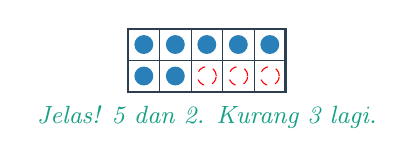
\begin{tikzpicture}[scale=0.4, baseline={([yshift=-.5ex]current bounding box.center)}]
            \draw[mainBlue, thin] (0,0) grid (5,2);
            \draw[mainBlue, thick] (0,0) rectangle (5,2);
            % Fill 7 organized
            \foreach \x in {0.5, 1.5, 2.5, 3.5, 4.5} \fill[dotBlue] (\x, 1.5) circle (0.3);
            \foreach \x in {0.5, 1.5} \fill[dotBlue] (\x, 0.5) circle (0.3);
            % Empty slots highlight
            \foreach \x in {2.5, 3.5, 4.5} \draw[dashed, red] (\x, 0.5) circle (0.3);
            
            % Caption inside tikzpicture
            \node[font=\small\itshape, text=accentTeal] at (2.5, -0.8) {Jelas! 5 dan 2. Kurang 3 lagi.};
        \end{tikzpicture}
    \end{minipage}
\end{tcolorbox}

% --- SECTION 2: ANATOMI ---
\begin{tcolorbox}[title=\textbf{2. ANATOMI \& FILOSOFI DESAIN}, colback=white, colframe=accentTeal, coltitle=white, fonttitle=\bfseries\large]
    \begin{minipage}{0.45\textwidth}
        \centering
        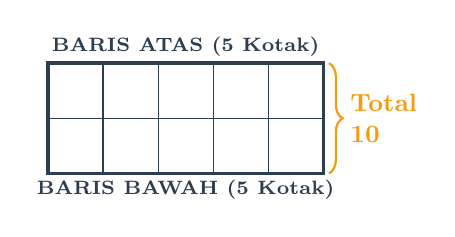
\begin{tikzpicture}[x=0.7cm, y=0.7cm, baseline={([yshift=-.5ex]current bounding box.center)}]
            \DrawFrame{0}{0}
            \node[font=\bfseries\scriptsize, text=mainBlue] at (2.5, 2.3) {BARIS ATAS (5 Kotak)};
            \node[font=\bfseries\scriptsize, text=mainBlue] at (2.5, -0.3) {BARIS BAWAH (5 Kotak)};
            \draw[decorate, decoration={brace, amplitude=5pt}, thick, color=niceOrange] (5.1, 2) -- (5.1, 0) node [midway, right=4pt, align=left, text=niceOrange, font=\bfseries\small] {Total\\10};
        \end{tikzpicture}
    \end{minipage}%
    \hfill
    \begin{minipage}{0.5\textwidth}
        \textbf{Logika Desain 2 x 5:}
        \begin{itemize}[leftmargin=*]
            \item Mengikuti pola jari tangan manusia (5 + 5).
            \item Otak sulit memproses >5 objek acak sekaligus. Ten Frame memecahnya menjadi bagian yang mudah dikelola (\textit{chunking}).
        \end{itemize}
    \end{minipage}
\end{tcolorbox}

% --- SECTION 3: JEMBATAN C-P-A ---
\begin{tcolorbox}[title=\textbf{3. JEMBATAN C-P-A (ALUR BELAJAR)}, colback=softBgA, colframe=niceOrange, coltitle=white, fonttitle=\bfseries\large]
    \centering
    \begin{tikzpicture}[node distance=0.2cm and 0.5cm]
        \node[conceptBox] (concrete) {
            \textbf{A. KONKRET}\\ \textit{"Benda Nyata"}\\
            \vspace{0.1cm}
            \begin{tikzpicture}[scale=0.4, baseline={([yshift=-0.5ex]current bounding box.center)}]
                \fill[dotBlue] (-1.2, 0.5) circle (0.3);
                \fill[dotBlue] (-0.3, 0.9) circle (0.3);
                \fill[dotBlue] (0.6, 0.4) circle (0.3);
                \fill[dotBlue] (1.4, 0.8) circle (0.3);
                \fill[dotBlue] (-0.7, -0.3) circle (0.3);
                \fill[dotBlue] (0.9, -0.5) circle (0.3);
            \end{tikzpicture}
        };
        \node[conceptBox, right=of concrete] (bridge) {
            \textbf{B. JEMBATAN}\\ \textit{"Masuk Frame"}\\
            \vspace{0.1cm}
            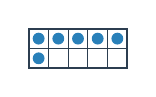
\begin{tikzpicture}[x=0.25cm, y=0.25cm] 
                \draw[mainBlue, thin, step=1] (0,0) grid (5,2);
                \draw[mainBlue, thick] (0,0) rectangle (5,2);
                \foreach \x in {0.5, 1.5, 2.5, 3.5, 4.5} \fill[dotBlue] (\x, 1.5) circle (0.3);
                \foreach \x in {0.5} \fill[dotBlue] (\x, 0.5) circle (0.3);
            \end{tikzpicture}
        };
        \node[conceptBox, right=of bridge] (pictorial) {
            \textbf{C. PIKTORIAL}\\ \textit{"Gambar Mental"}\\
            \vspace{0.1cm}
            \tikz{\node[cloud, cloud puffs=8, draw, fill=gray!10] {\textbf{"6"}};}
        };
        \draw[arrowFlow] (concrete) -- (bridge);
        \draw[arrowFlow] (bridge) -- (pictorial);
    \end{tikzpicture}
\end{tcolorbox}

\newpage

% --- TEN FRAME MASTERY CASES ---

\begin{tcolorbox}[colback=mainBlue, colframe=mainBlue, arc=0mm, boxrule=0pt, top=4mm, bottom=4mm, halign=center]
    {\Huge \bfseries \color{white} TEN FRAME MASTERY} \\
    \vspace{0.1cm}
    {\large \color{accentTeal} \textbf{Analisis Masalah \& Intervensi Visual}}
\end{tcolorbox}
\vspace{0.3cm}

\begin{CaseStudyBox}{KASUS 1: "SAYA HARUS HITUNG SATU-SATU DARI AWAL"}
\begin{minipage}{0.3\textwidth}
    \centering
    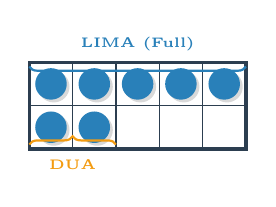
\begin{tikzpicture}[tfPic]
        \DrawFrame{0}{0}
        % Pattern 7: 5 top, 2 bottom
        \foreach \x in {0.5, 1.5, 2.5, 3.5, 4.5} \node[counter] at (\x, 1.5) {};
        \foreach \x in {0.5, 1.5} \node[counter] at (\x, 0.5) {};
        
        % Visual cue grouping
        \draw[decorate, decoration={brace, mirror, amplitude=3pt}, thick, powerBlue] (0, 1.9) -- (5, 1.9) node[midway, above=2pt, font=\tiny\bfseries] {LIMA (Full)};
        \draw[decorate, decoration={brace, amplitude=3pt}, thick, niceOrange] (0, 0.1) -- (2, 0.1) node[midway, below=2pt, font=\tiny\bfseries] {DUA};
    \end{tikzpicture}
\end{minipage}%
\hfill
\begin{minipage}{0.68\textwidth}
    \begin{itemize}[leftmargin=0.4cm, label={}]
        \item \textbf{\textcolor{alertRed}{Masalah (The Struggle):}} \textit{Counting All}. 
        Siswa melihat 7 benda. Otaknya tidak memproses "7" sebagai kesatuan, melainkan urutan "1, 2, 3, 4, 5, 6, 7".
        
        \item \textbf{\textcolor{powerBlue}{Kenapa Ten Frame?}} \textit{Structure as Anchor}.
        Ten Frame memaksa pengelompokan (subitizing). Baris atas penuh selalu berarti 5.
        
        \item \textbf{\textcolor{solGreen}{Solusi Intervensi:}}
        \textbf{"Flash Cards 2 Detik"}. Tunjukkan frame berisi 7 selama 2 detik lalu tutup. 
        \begin{itemize}[label=-, topsep=0pt, itemsep=0pt, font=\small]
            \item Tanya: "Apa yang kamu lihat?"
            \item Jawaban: "Saya lihat baris atas penuh (5) dan ada 2 di bawah. Jadi 7."
        \end{itemize}
    \end{itemize}
\end{minipage}
\end{CaseStudyBox}

\vspace{0.3cm}

\begin{CaseStudyBox}{KASUS 2: "SAYA LUPA PASANGAN ANGKA 10"}
\begin{minipage}{0.3\textwidth}
    \centering
    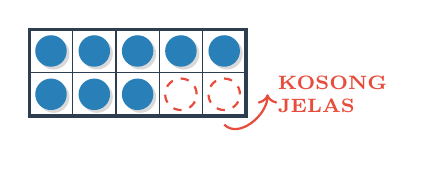
\begin{tikzpicture}[tfPic]
        \DrawFrame{0}{0}
        % 8 dots
        \foreach \x in {0.5, 1.5, 2.5, 3.5, 4.5} \node[counter] at (\x, 1.5) {};
        \foreach \x in {0.5, 1.5, 2.5} \node[counter] at (\x, 0.5) {};
        
        % 2 ghosts
        \node[ghostCounter] at (3.5, 0.5) {};
        \node[ghostCounter] at (4.5, 0.5) {};
        
        \draw[->, alertRed, thick] (4.5, -0.2) to[out=-45, in=-90] (5.5, 0.5) node[right, font=\scriptsize\bfseries, align=left] {KOSONG\\JELAS};
    \end{tikzpicture}
\end{minipage}%
\hfill
\begin{minipage}{0.68\textwidth}
    \begin{itemize}[leftmargin=0.4cm, label={}]
        \item \textbf{\textcolor{alertRed}{Masalah:}} \textit{Abstract Memorization}. 
        Siswa menghafal $8+2=10$ seperti puisi.
        
        \item \textbf{\textcolor{powerBlue}{Kenapa Ten Frame?}} \textit{Negative Space}.
        Mata manusia peka terhadap "kosong". Ten Frame memvisualisasikan "apa yang hilang".
        
        \item \textbf{\textcolor{solGreen}{Solusi Intervensi:}}
        \textbf{"Analogi Kursi Bus"}. 
        \begin{itemize}[label=-, topsep=0pt, itemsep=0pt, font=\small]
            \item "Bus kapasitas 10. Sudah naik 8 penumpang."
            \item "Berapa kursi kosong?" (Siswa menunjuk 2 kotak kosong).
        \end{itemize}
    \end{itemize}
\end{minipage}
\end{CaseStudyBox}

\vspace{0.3cm}

\begin{CaseStudyBox}{KASUS 3: "9 + 5 SUSAH, JARI SAYA CUMA 10"}
\begin{minipage}{0.3\textwidth}
    \centering
    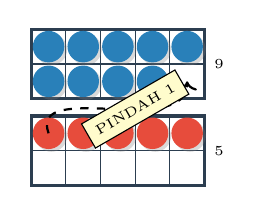
\begin{tikzpicture}[tfPic, scale=0.8]
        % Frame 9
        \DrawFrame{0}{2.5}
        \foreach \x in {0.5, 1.5, 2.5, 3.5, 4.5} \node[counter] at (\x, 4) {};
        \foreach \x in {0.5, 1.5, 2.5, 3.5} \node[counter] at (\x, 3) {};
        \node[right, font=\tiny] at (5, 3.5) {9};

        % Frame 5
        \DrawFrame{0}{0}
        \foreach \x in {0.5, 1.5, 2.5, 3.5, 4.5} \node[counterRed] at (\x, 1.5) {};
        \node[right, font=\tiny] at (5, 1) {5};
        
        % The Move
        \draw[->, black, dashed, thick] (0.5, 1.5) to[out=110, in=-90] (4.5, 3);
        \node[draw=black, fill=yellow!20, font=\tiny, align=center, rotate=30] at (3, 2.2) {PINDAH 1};
    \end{tikzpicture}
\end{minipage}%
\hfill
\begin{minipage}{0.68\textwidth}
    \begin{itemize}[leftmargin=0.4cm, label={}]
        \item \textbf{\textcolor{alertRed}{Masalah:}} \textit{Crossing the Ten}. 
        Bingung "menyimpan" angka di kepala.
        
        \item \textbf{\textcolor{powerBlue}{Kenapa Ten Frame?}} \textit{Decomposition}.
        Memecah 5 menjadi (1 + 4) untuk melengkapi 9.
        
        \item \textbf{\textcolor{solGreen}{Solusi Intervensi:}}
        \textbf{"Make a Ten Strategy"}.
        \begin{itemize}[label=-, topsep=0pt, itemsep=0pt, font=\small]
            \item "9 ingin jadi 10. Dia minta 1 dari 5."
            \item Visual: \textbf{1 frame penuh (10)} dan \textbf{sisa 4}.
            \item $9 + 5 \rightarrow 10 + 4 = 14$.
        \end{itemize}
    \end{itemize}
\end{minipage}
\end{CaseStudyBox}

\newpage

\begin{CaseStudyBox}{KASUS 4: "BERAPA LEBIHNYA 7 DARI 4?"}
\begin{minipage}{0.3\textwidth}
    \centering
    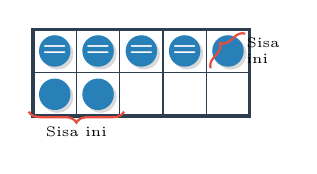
\begin{tikzpicture}[tfPic]
        \DrawFrame{0}{0}
        % 7 counters
        \foreach \x in {0.5, 1.5, 2.5, 3.5, 4.5} \node[counter] at (\x, 1.5) {};
        \foreach \x in {0.5, 1.5} \node[counter] at (\x, 0.5) {};
        
        % 4 counters (comparison)
        \foreach \x in {0.5, 1.5, 2.5, 3.5} \node[text=white, font=\bfseries] at (\x, 1.5) {=};
        
        \draw[decorate, decoration={brace, amplitude=4pt}, thick, alertRed] (4.1, 1.1) -- (4.9, 1.9) node[midway, right=3pt, font=\tiny, align=left, color=black] {Sisa\\ini};
        \draw[decorate, decoration={brace, amplitude=4pt, mirror}, thick, alertRed] (-0.1, 0.1) -- (2.1, 0.1) node[midway, below=2pt, font=\tiny, color=black] {Sisa ini};
    \end{tikzpicture}
\end{minipage}%
\hfill
\begin{minipage}{0.68\textwidth}
    \begin{itemize}[leftmargin=0.4cm, label={}]
        \item \textbf{\textcolor{alertRed}{Masalah:}} \textit{Comparison Concept}. 
        Kata "selisih" terdengar abstrak.
        
        \item \textbf{\textcolor{powerBlue}{Kenapa Ten Frame?}} \textit{Linear Alignment}.
        Grid memastikan posisi pasti untuk matching.
        
        \item \textbf{\textcolor{solGreen}{Solusi Intervensi:}}
        \textbf{"Pasang-Pasangkan"}. 
        \begin{itemize}[label=-, topsep=0pt, itemsep=0pt, font=\small]
            \item "Ayo kita jodohkan."
            \item Bagian yang "jomblo" atau tidak punya pasangan itulah bedanya.
        \end{itemize}
    \end{itemize}
\end{minipage}
\end{CaseStudyBox}

\vspace{0.3cm}

\begin{CaseStudyBox}{KASUS 5: "13 ITU APA? SATU DAN TIGA?"}
\begin{minipage}{0.3\textwidth}
    \centering
    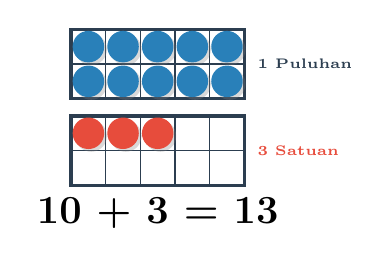
\begin{tikzpicture}[tfPic, scale=0.8]
        % Frame 10 (Full)
        \DrawFrame{0}{2.5}
        \foreach \x in {0.5, 1.5, 2.5, 3.5, 4.5} {
            \node[counter] at (\x, 4) {};
            \node[counter] at (\x, 3) {};
        }
        \node[font=\bfseries\tiny, color=mainBlue, anchor=west] at (5.1, 3.5) {1 Puluhan};

        % Frame 3 (Part)
        \DrawFrame{0}{0}
        \foreach \x in {0.5, 1.5, 2.5} \node[counterRed] at (\x, 1.5) {};
        \node[font=\bfseries\tiny, color=alertRed, anchor=west] at (5.1, 1) {3 Satuan};
        
        \node[font=\bfseries\Large] at (2.5, -0.8) {10 + 3 = 13};
    \end{tikzpicture}
\end{minipage}%
\hfill
\begin{minipage}{0.68\textwidth}
    \begin{itemize}[leftmargin=0.4cm, label={}]
        \item \textbf{\textcolor{alertRed}{Masalah:}} \textit{Place Value Confusion}. 
        Siswa melihat "13" sebagai digit "1" dan "3" terpisah.
        
        \item \textbf{\textcolor{powerBlue}{Kenapa Ten Frame?}} \textit{Unitizing Ten}.
        Visual ini membuktikan 1 frame penuh adalah "satu kelompok sepuluh".
        
        \item \textbf{\textcolor{solGreen}{Solusi Intervensi:}}
        \textbf{"Say Ten Counting"}.
        \begin{itemize}[label=-, topsep=0pt, itemsep=0pt, font=\small]
            \item Gunakan bahasa matematika: "Satu puluhan tiga satuan".
        \end{itemize}
    \end{itemize}
\end{minipage}
\end{CaseStudyBox}

\vspace{0.3cm}

\begin{CaseStudyBox}{KASUS 6: "LUPA MANA GANJIL MANA GENAP"}
\begin{minipage}{0.3\textwidth}
    \centering
    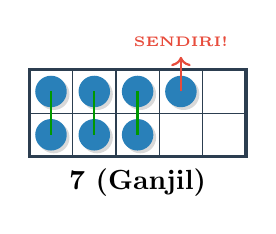
\begin{tikzpicture}[tfPic]
        \DrawFrame{0}{0}
        % 7 Counters
        \foreach \x in {0.5, 1.5, 2.5} {
            \node[counter] at (\x, 1.5) {}; 
            \node[counter] at (\x, 0.5) {}; 
            \draw[thick, green!60!black] (\x, 1.5) -- (\x, 0.5); % Pairing lines
        }
        % The odd one
        \node[counter] at (3.5, 1.5) {};
        
        \draw[->, alertRed, thick] (3.5, 1.5) -- (3.5, 2.3) node[above, font=\tiny\bfseries] {SENDIRI!};
        \node[font=\bfseries] at (2.5, -0.6) {7 (Ganjil)};
    \end{tikzpicture}
\end{minipage}%
\hfill
\begin{minipage}{0.68\textwidth}
    \begin{itemize}[leftmargin=0.4cm, label={}]
        \item \textbf{\textcolor{alertRed}{Masalah:}} \textit{Rote Memorization}. 
        Menghafal ganjil genap tanpa paham konsep.
        
        \item \textbf{\textcolor{powerBlue}{Kenapa Ten Frame?}} \textit{Pairing Structure}.
        Ten Frame disusun 2 baris (pair-wise). Sifat ganjil (ada sisa) terlihat instan.
        
        \item \textbf{\textcolor{solGreen}{Solusi Intervensi:}}
        \textbf{"Temukan Temannya"}.
        \begin{itemize}[label=-, topsep=0pt, itemsep=0pt, font=\small]
            \item Jika di akhir ada kancing yang tidak punya teman di bawahnya $\rightarrow$ GANJIL.
        \end{itemize}
    \end{itemize}
\end{minipage}
\end{CaseStudyBox}

\vspace{0.3cm}

\begin{CaseStudyBox}{KASUS 7: "14 - 6 ITU SULIT SEKALI"}
\begin{minipage}{0.3\textwidth}
    \centering
    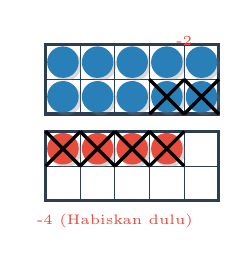
\begin{tikzpicture}[tfPic, scale=0.8]
        % Frame 10 (Full) with 2 crossed out
        \DrawFrame{0}{2.5}
        \foreach \x in {0.5, 1.5, 2.5} {
            \node[counter] at (\x, 4) {};
            \node[counter] at (\x, 3) {};
        }
        \foreach \x in {3.5, 4.5} {
            \node[counter] at (\x, 4) {};
            \node[counter] at (\x, 3) {};
        }
        % Cross out 2 from top frame
        \node[crossOut] at (4.5, 3) {};
        \node[crossOut] at (3.5, 3) {};
        \node[font=\tiny, color=alertRed] at (4, 4.6) {-2};

        % Frame 4 (Part) ALL crossed out
        \DrawFrame{0}{0}
        \foreach \x in {0.5, 1.5, 2.5, 3.5} {
            \node[counterRed] at (\x, 1.5) {};
            \node[crossOut] at (\x, 1.5) {};
        }
        \node[font=\tiny, color=alertRed] at (2, -0.6) {-4 (Habiskan dulu)};
    \end{tikzpicture}
\end{minipage}%
\hfill
\begin{minipage}{0.68\textwidth}
    \begin{itemize}[leftmargin=0.4cm, label={}]
        \item \textbf{\textcolor{alertRed}{Masalah:}} \textit{Hard Subtraction}. 
        $14 - 6$ menghitung mundur sering salah.
        
        \item \textbf{\textcolor{powerBlue}{Kenapa Ten Frame?}} \textit{Part-Part-Whole}.
        Strategi visual: Buang dulu sisa satuannya (4), baru ambil sisanya dari puluhan utuh.
        
        \item \textbf{\textcolor{solGreen}{Solusi Intervensi:}}
        \textbf{"Habiskan Ekornya Dulu"}.
        \begin{itemize}[label=-, topsep=0pt, itemsep=0pt, font=\small]
            \item "Buang dulu 4 yang di bawah." (Sisa mau buang 2 lagi).
            \item "Ambil 2 dari frame penuh."
            \item Siswa melihat sisa 8 di frame atas.
        \end{itemize}
    \end{itemize}
\end{minipage}
\end{CaseStudyBox}

\newpage

% =================================================================================
% BAGIAN 2: BLOK DIENES (BASE TEN BLOCKS)
% =================================================================================
\part{BLOK DIENES (NILAI TEMPAT)}

% --- HEADER ---
\begin{tcolorbox}[colback=mainBlue, colframe=mainBlue, arc=0mm, boxrule=0pt, top=5mm, bottom=5mm, halign=center]
    {\Huge \bfseries \color{white} BLOK DIENES (BASE TEN BLOCKS)} \\
    \vspace{0.2cm}
    {\large \color{accentTeal} \textbf{Visualisasi Konkret Nilai Tempat \& Algoritma}}
\end{tcolorbox}

\vspace{0.2cm}

% --- SECTION 1: KONTEKS MASALAH & SOLUSI ---
\begin{tcolorbox}[title=\textbf{1. KONTEKS: MENGAPA KITA BUTUH ALAT INI?}, colback=white, colframe=lightPurple, coltitle=white, fonttitle=\bfseries\large]
    \begin{minipage}[t]{0.48\textwidth}
        \textcolor{alertRed}{\Large \textbf{A. Masalah: "Abstract Symbols"}}
        \vspace{0.1cm}
        \begin{itemize}[leftmargin=*, itemsep=2pt]
            \item \textbf{Kebingungan Posisi:} Siswa melihat "2" pada angka "24" sama besarnya dengan "2" pada angka "2".
            \item \textbf{Tanpa Proporsi:} Simbol angka tidak menunjukkan ukuran (magnitude).
        \end{itemize}
    \end{minipage}%
    \hfill
    \begin{minipage}[t]{0.48\textwidth}
        \textcolor{accentTeal}{\Large \textbf{B. Solusi: Blok Dienes}}
        \vspace{0.1cm}
        \begin{itemize}[leftmargin=*, itemsep=2pt]
            \item \textbf{Proporsional:} Blok puluhan secara fisik \textbf{10x lebih besar} dari satuan.
            \item \textbf{Visualisasi Grup:} Memperjelas konsep "Satu Puluhan" adalah kumpulan "Sepuluh Satuan".
        \end{itemize}
    \end{minipage}
\end{tcolorbox}

% --- SECTION 2: ANATOMI ---
\begin{tcolorbox}[title=\textbf{2. ANATOMI: KONSISTENSI VISUAL 3D}, colback=white, colframe=accentTeal, coltitle=white, fonttitle=\bfseries\large]
    \centering
    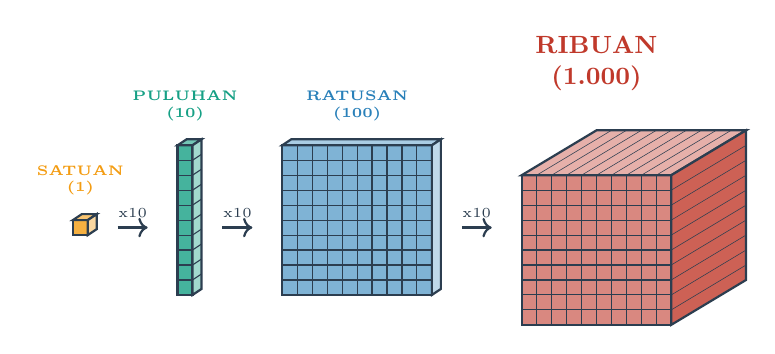
\begin{tikzpicture}[scale=0.38, baseline={([yshift=-.5ex]current bounding box.center)}]
        % Unit
        \DrawUnit{0}{3} 
        \node[above, font=\bfseries\tiny, text=niceOrange, align=center] at (0.25, 4) {SATUAN\\(1)};
        \draw[->, mainBlue, thick] (1.5, 3.25) -- (2.5, 3.25) node[midway, above, font=\tiny] {x10};
        
        % Long
        \DrawLong{3.5}{1} 
        \node[above, font=\bfseries\tiny, text=accentTeal, align=center] at (3.75, 6.5) {PULUHAN\\(10)};
        \draw[->, mainBlue, thick] (5, 3.25) -- (6, 3.25) node[midway, above, font=\tiny] {x10};
        
        % Flat
        \DrawFlat{7}{1} 
        \node[above, font=\bfseries\tiny, text=powerBlue, align=center] at (9.5, 6.5) {RATUSAN\\(100)};
        \draw[->, mainBlue, thick] (13, 3.25) -- (14, 3.25) node[midway, above, font=\tiny] {x10};
        
        % Cube
        \DrawThousand{15}{0} 
        \node[above, font=\bfseries\small, text=cubeRed, align=center] at (17.5, 7.5) {RIBUAN\\(1.000)};
    \end{tikzpicture}
    \vspace{0.2cm} \hrule \vspace{0.2cm}
    \begin{minipage}{0.9\textwidth}
        \textbf{Prinsip "Trading" (Tukar) Bertingkat:}
        \begin{itemize}[leftmargin=*, label=\checkbox]
            \item \textbf{10 Unit} $\rightarrow$ Tukar jadi \textbf{1 Long}.
            \item \textbf{10 Long} $\rightarrow$ Tukar jadi \textbf{1 Flat}.
            \item \textbf{10 Flat} $\rightarrow$ Tukar jadi \textbf{1 Cube}.
        \end{itemize}
    \end{minipage}
\end{tcolorbox}

% --- SECTION 3: JEMBATAN C-P-A ---
\begin{tcolorbox}[title=\textbf{3. JEMBATAN C-P-A (TRANSISI KE ABSTRAK)}, colback=softBgA, colframe=niceOrange, coltitle=white, fonttitle=\bfseries\large]
    \centering
    \begin{tikzpicture}[node distance=0.2cm and 0.5cm]
        \node[conceptBox] (concrete) {
            \textbf{A. KONKRET}\\ \textit{"Pegang Bloknya"}\\ \vspace{0.1cm}
            \begin{tikzpicture}[scale=0.2] \DrawLong{0}{0} \DrawUnit{1}{0} \DrawUnit{1}{0.7} \end{tikzpicture}
        };
        \node[conceptBox, right=of concrete] (bridge) {
            \textbf{B. PIKTORIAL}\\ \textit{"Gambar Sketsa"}\\ \vspace{0.1cm}
            
\begin{tikzpicture}[scale=0.25] \draw[thick, mainBlue] (0,0) -- (0,5); \fill[mainBlue] (1,0.5) circle (0.2); \fill[mainBlue] (1.5,0.5) circle (0.2); \end{tikzpicture}
        };
        \node[conceptBox, right=of bridge] (pictorial) {
            \textbf{C. ABSTRAK}\\ \textit{"Simbol Angka"}\\ \vspace{0.1cm}
            \tikz{\node[cloud, cloud puffs=8, draw, fill=gray!10, font=\bfseries\Large] {12};}
        };
        \draw[arrowFlow] (concrete) -- (bridge); \draw[arrowFlow] (bridge) -- (pictorial);
    \end{tikzpicture}
\end{tcolorbox}

\newpage

% --- DIENES MASTERY CASES ---

\begin{tcolorbox}[colback=mainBlue, colframe=mainBlue, arc=0mm, boxrule=0pt, top=4mm, bottom=4mm, halign=center]
    {\Huge \bfseries \color{white} DIENES MASTERY} \\
    \vspace{0.1cm}
    {\large \color{accentTeal} \textbf{Bedah Konsep Operasi Bilangan}}
\end{tcolorbox}
\vspace{0.3cm}

\begin{CaseStudyBox}{KASUS 1: MAGNITUDE "24 vs 42"}
\begin{minipage}{0.4\textwidth}
    \centering
    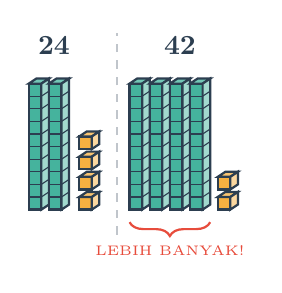
\begin{tikzpicture}[blockPic, scale=0.8]
        % 24 Area
        \node[font=\bfseries, mainBlue] at (1, 6.5) {24};
        \DrawLong{0}{0} \DrawLong{0.8}{0}
        \foreach \y in {0,1,2,3} \DrawUnit{2}{\y*0.8};
        
        % Separator
        \draw[dashed, mainBlue!30] (3.5, -1) -- (3.5, 7);

        % 42 Area
        \node[font=\bfseries, mainBlue] at (6, 6.5) {42};
        \DrawLong{4}{0} \DrawLong{4.8}{0} \DrawLong{5.6}{0} \DrawLong{6.4}{0}
        \foreach \y in {0,1} \DrawUnit{7.5}{\y*0.8};
        
        % Visual Cue
        \draw[decorate, decoration={brace, mirror, amplitude=5pt}, thick, alertRed] (4, -0.5) -- (7.2, -0.5) node[midway, below=5pt, font=\tiny] {LEBIH BANYAK!};
    \end{tikzpicture}
\end{minipage}%
\hfill
\begin{minipage}{0.58\textwidth}
    \textbf{Visualisasi:} Dengan memberikan efek 3D, siswa melihat bahwa 4 batang puluhan pada "42" secara fisik menempati ruang (volume) yang jauh lebih besar daripada 2 batang puluhan pada "24".
\end{minipage}
\end{CaseStudyBox}

\vspace{0.3cm}

\begin{CaseStudyBox}{KASUS 2: PENJUMLAHAN MENYIMPAN ($18 + 5$)}
\begin{minipage}{0.45\textwidth}
    \centering
    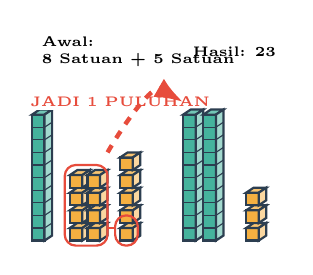
\begin{tikzpicture}[blockPic, scale=0.8] 
        % Context
        \node[font=\bfseries\tiny, anchor=west, align=left] at (0, 7.5) {Awal:\\8 Satuan + 5 Satuan};
        \DrawLong{0}{0} 
        
        % 8 units
        \foreach \y in {0,...,3} \DrawUnit{1.5}{\y*0.7};
        \foreach \y in {0,...,3} \DrawUnit{2.2}{\y*0.7};
        
        % 5 units (additions)
        \foreach \y in {0,...,4} \DrawUnit{3.5}{\y*0.7};
        
        % Grouping Ring (Circle 10 units)
        \draw[alertRed, thick, rounded corners] (1.3, -0.2) rectangle (3.0, 3.0); 
        \draw[alertRed, thick, rounded corners] (3.3, -0.2) rectangle (4.2, 1.0); 
        \draw[alertRed, thick] (3.0, 0.5) -- (3.3, 0.5); 
        
        % Label moved to (3.5, 5.5) with white background to prevent clutter
        \node[font=\bfseries\tiny, text=alertRed, fill=white, inner sep=1pt] at (3.5, 5.5) {JADI 1 PULUHAN};
        
        % Arrow start from grouping box top (y=3.5) to destination
        \draw[arrowOp, ultra thick] (3, 3.5) to[out=60, in=150] (6.0, 5.5);
        
        % Result - Moved Higher to y=7.5
        \node[font=\bfseries\tiny, anchor=west] at (6.0, 7.5) {Hasil: 23};
        \DrawLong{6.0}{0} \DrawLong{6.8}{0} % 2 Tens
        \foreach \y in {2,3,4} \DrawUnit{8.5}{\y*0.7 - 1.4}; % 3 remaining units
    \end{tikzpicture}
\end{minipage}%
\hfill
\begin{minipage}{0.52\textwidth}
    \textbf{Konsep:} "Bundling". Ketika satuan menumpuk lebih dari 9, visualisasikan ikatan merah yang menyatukan 10 satuan menjadi 1 batang utuh baru.
\end{minipage}
\end{CaseStudyBox}

\vspace{0.3cm}

\begin{CaseStudyBox}{KASUS 3: PENGURANGAN MEMINJAM ($32 - 15$)}
\begin{minipage}{0.45\textwidth}
    \centering
    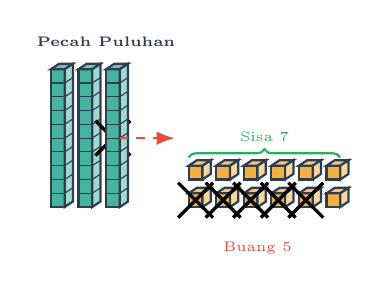
\begin{tikzpicture}[scale=0.35, baseline={([yshift=-.5ex]current bounding box.center)}]
        \node[font=\bfseries\tiny, mainBlue] at (2, 6) {Pecah Puluhan};
        % 3 Tens initially
        \DrawLong{0}{0} \DrawLong{1}{0} 
        % Exploded Ten
        \node[crossOut] at (2.25, 2.5) {}; 
        \DrawLong{2}{0}
        
        \draw[arrowOp] (2.5, 2.5) -- (4.5, 2.5);
        
        % The exploded units
        \foreach \y in {0,1} \foreach \x in {5,6,7,8,9} \DrawUnit{\x}{\y};
        
        % The original 2 units
        \DrawUnit{10}{0} \DrawUnit{10}{1}
        
        % Subtract 5 (Cross out)
        \foreach \x in {5,6,7,8,9} \node[crossOut] at (\x.25, 0.25) {};
        \node[font=\tiny, text=alertRed] at (7.5, -1.5) {Buang 5};
        
        % Brace showing result
        \draw[decorate, decoration={brace, amplitude=3pt}, thick, solGreen] (5, 1.8) -- (10.5, 1.8) node[midway, above=2pt, font=\tiny] {Sisa 7};
    \end{tikzpicture}
\end{minipage}%
\hfill
\begin{minipage}{0.52\textwidth}
    \textbf{Konsep:} "Unbundling/Decompose". Jangan gunakan istilah "pinjam" (karena tidak dikembalikan), gunakan "Tukar" atau "Pecah". Visualisasikan 1 batang hancur menjadi 10 keping.
\end{minipage}
\end{CaseStudyBox}

\vspace{0.3cm}

\begin{CaseStudyBox}{KASUS 4: PERKALIAN AREA DISTRIBUTIF ($12 \times 3$)}
\begin{minipage}{0.45\textwidth}
    \centering
    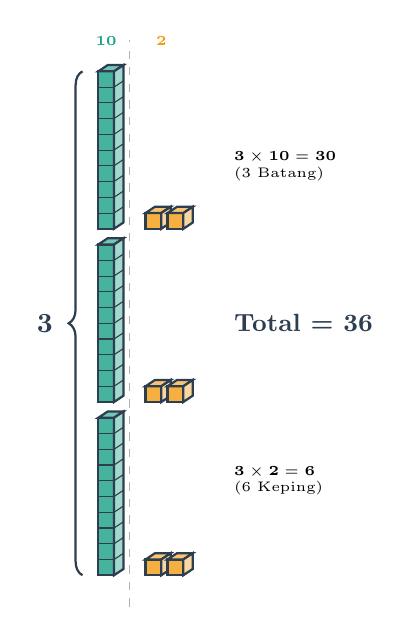
\begin{tikzpicture}[scale=0.4, baseline={([yshift=-.5ex]current bounding box.center)}]
        % Row 1
        \DrawLong{0}{0} \DrawUnit{1.5}{0} \DrawUnit{2.2}{0}
        % Row 2
        \DrawLong{0}{5.5} \DrawUnit{1.5}{5.5} \DrawUnit{2.2}{5.5}
        % Row 3
        \DrawLong{0}{11} \DrawUnit{1.5}{11} \DrawUnit{2.2}{11}

        % Grouping Braces
        \draw[decorate, decoration={brace, amplitude=5pt}, thick, mainBlue] (-0.5, 0) -- (-0.5, 16) node[midway, left=7pt, font=\bfseries] {3};
        
        % Top Labels showing distribution
        \node[above, font=\bfseries\tiny, text=accentTeal] at (0.25, 16.5) {10};
        \node[above, font=\bfseries\tiny, text=niceOrange] at (2, 16.5) {2};
        
        % Calculation
        \node[right, align=left, font=\tiny] at (4, 13) {$\mathbf{3 \times 10 = 30}$\\(3 Batang)};
        \node[right, align=left, font=\tiny] at (4, 3) {$\mathbf{3 \times 2 = 6}$\\(6 Keping)};
        \node[right, font=\bfseries\small, mainBlue] at (4, 8) {Total = 36};
        
        % Separation Line
        \draw[dashed, mainBlue!40] (1.0, -1) -- (1.0, 17);
    \end{tikzpicture}
\end{minipage}%
\hfill
\begin{minipage}{0.52\textwidth}
    \textbf{Konsep:} "Area Model". Pisahkan secara visual kolom puluhan dan kolom satuan. Ini membangun pondasi mental untuk aljabar $(x + 2)$ dan perkalian bersusun ke bawah.
\end{minipage}
\end{CaseStudyBox}

\vspace{0.3cm}

\begin{CaseStudyBox}{KASUS 5: PEMBAGIAN PARTISI ($42 \div 3$)}
\begin{minipage}{0.45\textwidth}
    \centering
    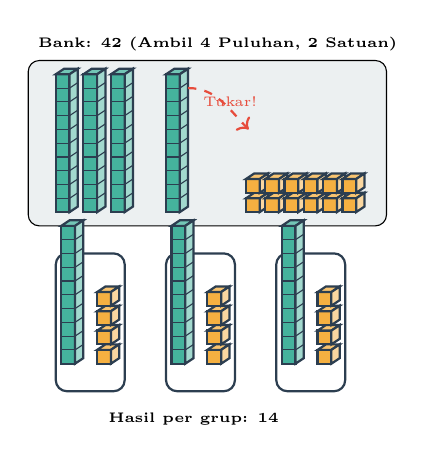
\begin{tikzpicture}[scale=0.35, baseline={([yshift=-.5ex]current bounding box.center)}]
        % --- BANK UTAMA ---
        \draw[fill=softBgA, rounded corners] (-1, 5) rectangle (12, 11);
        \node[anchor=south west, font=\tiny\bfseries] at (-1, 11) {Bank: 42 (Ambil 4 Puluhan, 2 Satuan)};
        
        % 3 Tens easy distribute
        \DrawLong{0}{5.5} \DrawLong{1}{5.5} \DrawLong{2}{5.5}
        
        % The Remainder Ten (At x=4)
        \DrawLong{4}{5.5}
        
        % Arrow moved to avoid text overlap
        \draw[->, thick, alertRed, dashed] (4.8, 10) to[out=0, in=135] (7, 8.5);
        
        % Text moved to the RIGHT of the block (x=5.0)
        \node[font=\tiny, text=alertRed, anchor=west] at (5.0, 9.5) {Tukar!};
        
        % Converted Units
        \foreach \y in {0,1} \foreach \x in {7,8,9,10,11,12} \DrawUnit{\x*0.7 + 2}{\y*0.7 + 5.5};
        
        % --- GROUPING BOXES ---
        \foreach \gx/\lbl in {0/A, 4/B, 8/C} {
            \draw[mainBlue, thick, rounded corners] (\gx, -1) rectangle (\gx+2.5, 4);
            % Distributed Ten
            \DrawLong{\gx+0.2}{0}
            % Distributed Units (4 per box)
            \foreach \uy in {0,1,2,3} \DrawUnit{\gx+1.5}{\uy*0.7};
        }
        \node[font=\bfseries\tiny] at (5, -2) {Hasil per grup: 14};

    \end{tikzpicture}
\end{minipage}%
\hfill
\begin{minipage}{0.52\textwidth}
    \textbf{Konsep:} "Partisi Adil".
    1. Bagi puluhan yang utuh dulu (3 batang ke 3 kotak).
    2. Sisa 1 batang tidak bisa dibagi $\rightarrow$ Tukar jadi 10 keping.
    3. Gabung dengan 2 keping awal (Total 12 keping).
    4. Bagi 12 keping ke 3 kotak (4 per kotak).
\end{minipage}
\end{CaseStudyBox}

\vspace{0.3cm}

\begin{CaseStudyBox}{KASUS 6: DESIMAL (1.23) - REDEFINISI "SATU"}
\begin{minipage}{0.45\textwidth}
    \centering
    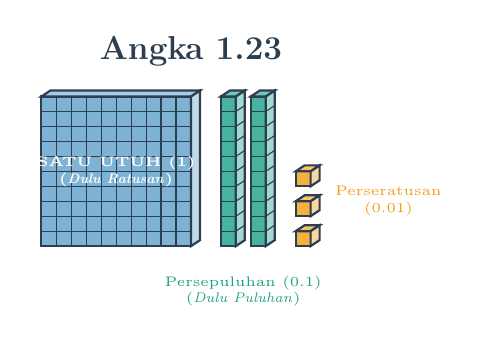
\begin{tikzpicture}[scale=0.38, baseline={([yshift=-.5ex]current bounding box.center)}]
        % The Whole (1)
        \DrawFlat{0}{0}
        \node[font=\bfseries\tiny, text=white, align=center] at (2.5, 2.5) {SATU UTUH (1)\\(\textit{Dulu Ratusan})};
        
        % The Tenths (0.1)
        \DrawLong{6}{0} \DrawLong{7}{0}
        \node[font=\tiny, text=accentTeal, align=center] at (6.75, -1.5) {Persepuluhan (0.1)\\(\textit{Dulu Puluhan})};
        
        % The Hundredths (0.01)
        \DrawUnit{8.5}{0} \DrawUnit{8.5}{1} \DrawUnit{8.5}{2}
        
        % MOVED LABEL TO THE RIGHT (avoid overlap)
        \node[font=\tiny, text=niceOrange, align=center, anchor=west] at (9.5, 1.5) {Perseratusan\\(0.01)};
        
        \node[font=\bfseries\large, mainBlue] at (5, 6.5) {Angka 1.23};
    \end{tikzpicture}
\end{minipage}%
\hfill
\begin{minipage}{0.52\textwidth}
    \textbf{Konsep:} "Relativitas Unit".
    Siswa sering bingung desimal karena menganggap kubus kecil *selalu* 1. 
    Ubah definisi: "Jika Keping Besar ini adalah 1 Kue Utuh, maka 1 Batang adalah potongannya (0.1), dan Kubus Kecil adalah remahannya (0.01)."
\end{minipage}
\end{CaseStudyBox}

\vspace{0.3cm}

\begin{CaseStudyBox}{KASUS 7: TRANSISI ALJABAR $(x+2)(x+1)$}
\begin{minipage}{0.45\textwidth}
    \centering
    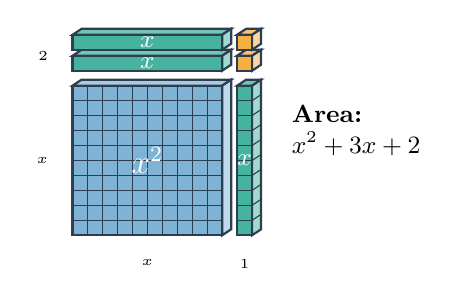
\begin{tikzpicture}[scale=0.38, baseline={([yshift=-.5ex]current bounding box.center)}]
        % x^2 (Flat)
        \DrawFlat{0}{0}
        \node[font=\bfseries\large, text=white] at (2.5, 2.5) {$x^2$};
        
        % x terms (Vertical Longs)
        \DrawLong{5.5}{0}
        \node[font=\bfseries\small, text=white] at (5.75, 2.5) {$x$};
        
        % x terms (Horizontal Longs - simulated by rotating dimensions manually)
        \begin{scope}[shift={(0,5.5)}]
             \draw[fill=accentTeal!80, draw=mainBlue, thick] (0,0) rectangle (5, 0.5);
             \draw[fill=accentTeal!60, draw=mainBlue, thick] (0,0.5) -- (0.3, 0.7) -- (5.3, 0.7) -- (5, 0.5) -- cycle;
             \draw[fill=accentTeal!40, draw=mainBlue, thick] (5,0) -- (5.3, 0.2) -- (5.3, 0.7) -- (5, 0.5) -- cycle;
             \node[font=\bfseries\small, text=white] at (2.5, 0.25) {$x$};
        \end{scope}
        \begin{scope}[shift={(0,6.2)}]
             \draw[fill=accentTeal!80, draw=mainBlue, thick] (0,0) rectangle (5, 0.5);
             \draw[fill=accentTeal!60, draw=mainBlue, thick] (0,0.5) -- (0.3, 0.7) -- (5.3, 0.7) -- (5, 0.5) -- cycle;
             \draw[fill=accentTeal!40, draw=mainBlue, thick] (5,0) -- (5.3, 0.2) -- (5.3, 0.7) -- (5, 0.5) -- cycle;
             \node[font=\bfseries\small, text=white] at (2.5, 0.25) {$x$};
        \end{scope}
        
        % Unit terms (1) filling the corner
        \DrawUnit{5.5}{5.5}
        \DrawUnit{5.5}{6.2}
        
        % Labels
        \node[left, font=\bfseries\tiny] at (-0.5, 2.5) {$x$};
        \node[left, font=\bfseries\tiny] at (-0.5, 6) {$2$};
        \node[below, font=\bfseries\tiny] at (2.5, -0.5) {$x$};
        \node[below, font=\bfseries\tiny] at (5.75, -0.5) {$1$};
        
        \node[align=left, font=\bfseries\small, anchor=west] at (7, 3.5) {Area:\\$x^2 + 3x + 2$};
    \end{tikzpicture}
\end{minipage}%
\hfill
\begin{minipage}{0.52\textwidth}
    \textbf{Konsep:} "Aljabar Geometris".
    Blok Dienes bukan hanya untuk aritmatika.
    Gunakan "Flat" sebagai $x^2$ (ukuran tak tentu), "Long" sebagai $x$, dan "Unit" sebagai 1.
    Ini membuktikan secara visual bahwa $(x+2)(x+1) = x^2 + 3x + 2$.
\end{minipage}
\end{CaseStudyBox}

\newpage

% =================================================================================
% BAGIAN 3: BAR MODEL (SINGAPORE MATH)
% =================================================================================
\part{SINGAPORE BAR MODEL (PROBLEM SOLVING)}

% --- HEADER ---
\begin{tcolorbox}[colback=mainBlue, colframe=mainBlue, arc=0mm, boxrule=0pt, top=5mm, bottom=5mm, halign=center]
    {\Huge \bfseries \color{white} SINGAPORE BAR MODEL} \\
    \vspace{0.2cm}
    {\large \color{accentTeal} \textbf{Jembatan Visual Soal Cerita ke Aljabar}}
\end{tcolorbox}

\vspace{0.5cm}

% --- SECTION 1: KONTEKS MASALAH & SOLUSI ---
\begin{tcolorbox}[title=\textbf{1. FILOSOFI: MENGAPA BAR MODEL?}, colback=white, colframe=lightPurple, coltitle=white, fonttitle=\bfseries\large]
    \begin{minipage}[t]{0.48\textwidth}
        \textcolor{alertRed}{\Large \textbf{A. Masalah: "Lost in Translation"}}
        \vspace{0.1cm}
        \begin{itemize}[leftmargin=*, itemsep=2pt]
            \item \textbf{Abstraksi Dini:} Siswa kesulitan langsung mengubah kalimat cerita menjadi persamaan matematika ($x + y = z$).
            \item \textbf{Struktur Tersembunyi:} Hubungan antar besaran (lebih banyak, selisih, total) tidak terlihat dalam teks.
        \end{itemize}
    \end{minipage}%
    \hfill
    \begin{minipage}[t]{0.48\textwidth}
        \textcolor{accentTeal}{\Large \textbf{B. Solusi: Representasi Piktorial}}
        \vspace{0.1cm}
        \begin{itemize}[leftmargin=*, itemsep=2pt]
            \item \textbf{Visualisasi Kuantitas:} Panjang batang merepresentasikan nilai (magnitude).
            \item \textbf{Visualisasi Relasi:} Posisi batang (berderet atau bertumpuk) menunjukkan hubungan penjumlahan atau perbandingan.
        \end{itemize}
    \end{minipage}
\end{tcolorbox}

% --- SECTION 2: ANATOMI ---
\begin{tcolorbox}[title=\textbf{2. ANATOMI BAR MODEL}, colback=white, colframe=accentTeal, coltitle=white, fonttitle=\bfseries\large]
    \centering
    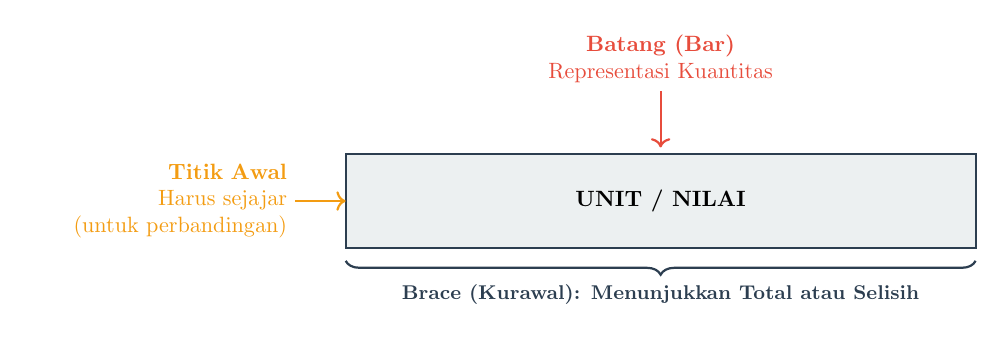
\begin{tikzpicture}[scale=0.8, transform shape]
        % Main Bar
        \draw[fill=softBgA, draw=mainBlue, thick] (0,0) rectangle (10, 1.5);
        
        % Labels inside
        \node at (5, 0.75) {\textbf{UNIT / NILAI}};
        
        % Anatomy annotations
        \draw[<-, thick, alertRed] (5, 1.6) -- (5, 2.5) node[above, align=center] {\textbf{Batang (Bar)}\\Representasi Kuantitas};
        \draw[<-, thick, niceOrange] (0, 0.75) -- (-0.8, 0.75) node[left, align=right, text width=4cm] {\textbf{Titik Awal}\\Harus sejajar\\(untuk perbandingan)};
        
        % Brace
        \DrawBraceDown{0}{10}{-0.2}{Brace (Kurawal): Menunjukkan Total atau Selisih}
    \end{tikzpicture}
    \vspace{0.2cm} \hrule \vspace{0.2cm}
    \begin{minipage}{0.9\textwidth}
        \textbf{Prinsip Dasar:}
        \begin{itemize}[leftmargin=*, label=\checkbox]
            \item \textbf{Panjang Proporsional:} Nilai yang lebih besar digambar lebih panjang (sketsa, tidak perlu presisi milimeter).
            \item \textbf{Konservasi:} Batang bisa dipotong, digeser, atau digabung tanpa mengubah nilai totalnya.
        \end{itemize}
    \end{minipage}
\end{tcolorbox}

% --- SECTION 3: C-P-A BRIDGE ---
\begin{tcolorbox}[title=\textbf{3. TRANSISI C-P-A (PENGENALAN ALJABAR)}, colback=softBgA, colframe=niceOrange, coltitle=white, fonttitle=\bfseries\large]
    \centering
    \begin{tikzpicture}[node distance=0.2cm and 0.5cm]
        \node[conceptBox] (concrete) {
            \textbf{A. KONKRET}\\ \textit{3 Keranjang "x"}\\ \vspace{0.1cm}
            \begin{tikzpicture}[scale=0.4, baseline=0] 
                % Basket 1
                \begin{scope}[shift={(0,0)}]
                    \draw[thick, mainBlue] (0.1,0.2) to[out=110, in=70] (1.4,0.2);
                    \draw[fill=niceOrange!40, draw=mainBlue, thick] (0,0.2) -- (0.25,-0.6) -- (1.25,-0.6) -- (1.5,0.2) -- cycle;
                    \node[font=\bfseries\large, mainBlue] at (0.75, -0.2) {$x$};
                \end{scope}
                % Basket 2
                \begin{scope}[shift={(1.8,0)}]
                    \draw[thick, mainBlue] (0.1,0.2) to[out=110, in=70] (1.4,0.2);
                    \draw[fill=niceOrange!40, draw=mainBlue, thick] (0,0.2) -- (0.25,-0.6) -- (1.25,-0.6) -- (1.5,0.2) -- cycle;
                    \node[font=\bfseries\large, mainBlue] at (0.75, -0.2) {$x$};
                \end{scope}
                % Basket 3
                \begin{scope}[shift={(3.6,0)}]
                    \draw[thick, mainBlue] (0.1,0.2) to[out=110, in=70] (1.4,0.2);
                    \draw[fill=niceOrange!40, draw=mainBlue, thick] (0,0.2) -- (0.25,-0.6) -- (1.25,-0.6) -- (1.5,0.2) -- cycle;
                    \node[font=\bfseries\large, mainBlue] at (0.75, -0.2) {$x$};
                \end{scope}
            \end{tikzpicture}
        };
        \node[conceptBox, right=of concrete] (pictorial) {
            \textbf{B. PIKTORIAL}\\ \textit{3 Himpunan Variabel}\\ \vspace{0.1cm}
            
\begin{tikzpicture}[scale=0.5, baseline=-5] 
                % Circle 1
                \draw[thick, mainBlue, fill=white] (0, 0) circle (0.6);
                \node[font=\bfseries\large, mainBlue, anchor=center] at (0, 0) {$x$};
                
                % Circle 2
                \draw[thick, mainBlue, fill=white] (1.5, 0) circle (0.6);
                \node[font=\bfseries\large, mainBlue, anchor=center] at (1.5, 0) {$x$};
                
                % Circle 3
                \draw[thick, mainBlue, fill=white] (3.0, 0) circle (0.6);
                \node[font=\bfseries\large, mainBlue, anchor=center] at (3.0, 0) {$x$};
            \end{tikzpicture}
        };
        \node[conceptBox, right=of pictorial] (abstract) {
            \textbf{C. ABSTRAK}\\ \textit{Aljabar}\\ \vspace{0.1cm}
            \tikz{\node[font=\bfseries\Huge, color=mainBlue] {3x};}
        };
        \draw[arrowFlow] (concrete) -- (pictorial); 
        \draw[arrowFlow] (pictorial) -- (abstract);
    \end{tikzpicture}
\end{tcolorbox}

\newpage

% --- EMPAT LOGIKA UTAMA ---
\begin{tcolorbox}[colback=mainBlue, colframe=mainBlue, arc=0mm, boxrule=0pt, top=4mm, bottom=4mm, halign=center]
    {\Huge \bfseries \color{white} STRUKTUR DASAR} \\
    \vspace{0.1cm}
    {\large \color{accentTeal} \textbf{Empat Logika Utama Bar Model}}
\end{tcolorbox}
\vspace{0.3cm}

% --- TYPE 1: PART-WHOLE ---
\begin{ConceptBox}{TIPE 1: PART-WHOLE MODEL (Bagian-Keseluruhan)}
\begin{minipage}{0.45\textwidth}
    \centering
    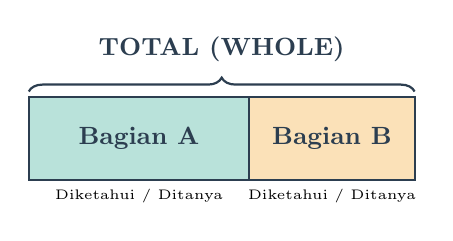
\begin{tikzpicture}[scale=0.7]
        % Whole Bar split into two
        \draw[fill=accentTeal!30, draw=mainBlue, thick] (0,0) rectangle (4, 1.5);
        \draw[fill=niceOrange!30, draw=mainBlue, thick] (4,0) rectangle (7, 1.5);
        
        % Labels
        \node[modelLabel] at (2, 0.75) {Bagian A};
        \node[modelLabel] at (5.5, 0.75) {Bagian B};
        
        % Braces
        \DrawBraceUp{0}{7}{1.6}{TOTAL (WHOLE)}
        \node[font=\tiny, below] at (2,0) {Diketahui / Ditanya};
        \node[font=\tiny, below] at (5.5,0) {Diketahui / Ditanya};
    \end{tikzpicture}
\end{minipage}%
\hfill
\begin{minipage}{0.5\textwidth}
    \textbf{Kapan Digunakan?}
    \begin{itemize}[leftmargin=*, itemsep=2pt]
        \item Operasi Penjumlahan (Mencari Total).
        \item Operasi Pengurangan (Diketahui Total dan satu Bagian, mencari Bagian lain).
        \item Tidak ada perbandingan "lebih banyak/sedikit".
    \end{itemize}
    \textit{Contoh Kalimat: "A dan B digabungkan...", "Sebagian adalah A, sisanya B..."}
\end{minipage}
\end{ConceptBox}

\vspace{0.3cm}

% --- TYPE 2: COMPARISON ---
\begin{ConceptBox}{TIPE 2: COMPARISON MODEL (Perbandingan)}
\begin{minipage}{0.45\textwidth}
    \centering
    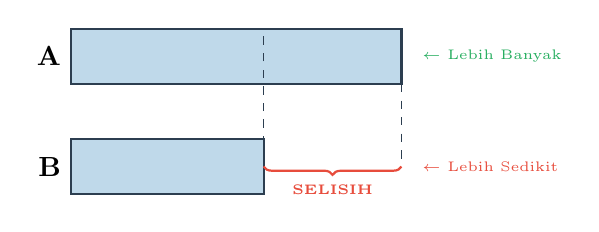
\begin{tikzpicture}[scale=0.7]
        % Bar A
        \node[left, font=\bfseries] at (0, 2.5) {A};
        \draw[fill=powerBlue!30, draw=mainBlue, thick] (0,2) rectangle (6, 3);
        
        % Bar B (Shorter)
        \node[left, font=\bfseries] at (0, 0.5) {B};
        \draw[fill=powerBlue!30, draw=mainBlue, thick] (0,0) rectangle (3.5, 1);
        
        % Dotted lines for comparison
        \draw[dashed, mainBlue] (3.5, 0) -- (3.5, 3);
        \draw[dashed, mainBlue] (6, 2) -- (6, 0.5);
        
        % Difference Brace
        \draw[decorate, decoration={brace, mirror, amplitude=3pt}, thick, alertRed] (3.5, 0.5) -- (6, 0.5) node[midway, below=3pt, font=\bfseries\tiny] {SELISIH};
        
        % Comparison logic - MOVED TO THE RIGHT TO AVOID COLLISION
        \node[font=\tiny, anchor=west, text=solGreen] at (6.2, 2.5) {$\leftarrow$ Lebih Banyak};
        \node[font=\tiny, anchor=west, text=alertRed] at (6.2, 0.5) {$\leftarrow$ Lebih Sedikit};
    \end{tikzpicture}
\end{minipage}%
\hfill
\begin{minipage}{0.5\textwidth}
    \textbf{Kapan Digunakan?}
    \begin{itemize}[leftmargin=*, itemsep=2pt]
        \item Membandingkan dua entitas berbeda.
        \item Kata kunci: "Lebih banyak dari", "Lebih sedikit dari", "Berapa bedanya", "Sama banyak dengan".
    \end{itemize}
    \textbf{Konsep Kunci:} Alignment (Kesejajaran) di sisi kiri sangat krusial untuk melihat selisih di sisi kanan.
\end{minipage}
\end{ConceptBox}

\vspace{0.3cm}

% --- TYPE 3: EQUAL PARTS / MULTIPLICATION ---
\begin{ConceptBox}{TIPE 3: EQUAL PARTS (Perkalian \& Pembagian)}
\begin{minipage}{0.45\textwidth}
    \centering
    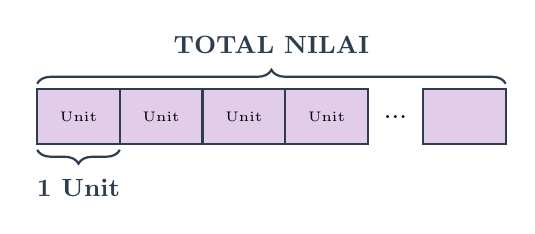
\begin{tikzpicture}[scale=0.7]
        % Bar split into equal parts
        \foreach \x in {0, 1.5, 3, 4.5} {
            \draw[fill=lightPurple!30, draw=mainBlue, thick] (\x, 0) rectangle (\x+1.5, 1);
            \node[font=\tiny] at (\x+0.75, 0.5) {Unit};
        }
        
        % Dot dot dot implies many
        \node at (6.5, 0.5) {...};
        \draw[fill=lightPurple!30, draw=mainBlue, thick] (7, 0) rectangle (8.5, 1);
        
        % Braces
        \DrawBraceDown{0}{1.5}{-0.1}{1 Unit}
        \DrawBraceUp{0}{8.5}{1.1}{TOTAL NILAI}
        
    \end{tikzpicture}
\end{minipage}%
\hfill
\begin{minipage}{0.5\textwidth}
    \textbf{Kapan Digunakan?}
    \begin{itemize}[leftmargin=*, itemsep=2pt]
        \item Benda-benda identik dalam jumlah banyak.
        \item Pecahan (Fraction): 1 bagian dari 5 bagian yang sama.
        \item Rasio (Perbandingan Senilai): 3 kotak vs 2 kotak.
    \end{itemize}
    \textbf{Konsep Kunci:} "Unitary Method". Mencari nilai \textbf{1 Unit} adalah kunci untuk memecahkan seluruh masalah.
\end{minipage}
\end{ConceptBox}

\vspace{0.3cm}

% --- TYPE 4: BEFORE-AFTER / CHANGE ---
\begin{ConceptBox}{TIPE 4: CHANGE MODEL (Perubahan/Transformasi)}
\begin{minipage}{0.45\textwidth}
    \centering
    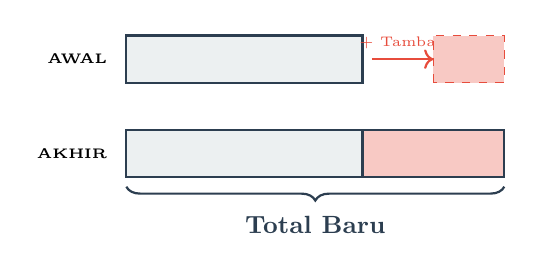
\begin{tikzpicture}[scale=0.6]
        % Before
        \node[anchor=east, font=\bfseries\tiny] at (-0.2, 2.5) {AWAL};
        \draw[fill=softBgA, draw=mainBlue, thick] (0,2) rectangle (5, 3);
        
        % Operation Arrow
        \draw[->, thick, alertRed] (5.2, 2.5) -- (6.5, 2.5) node[midway, above, font=\tiny] {+ Tambah};
        \draw[fill=alertRed!30, draw=alertRed, dashed] (6.5, 2) rectangle (8, 3);
        
        % After
        \node[anchor=east, font=\bfseries\tiny] at (-0.2, 0.5) {AKHIR};
        \draw[fill=softBgA, draw=mainBlue, thick] (0,0) rectangle (5, 1);
        \draw[fill=alertRed!30, draw=mainBlue, thick] (5,0) rectangle (8, 1);
        
        % Brace showing new total
        \DrawBraceDown{0}{8}{-0.2}{Total Baru}
    \end{tikzpicture}
\end{minipage}%
\hfill
\begin{minipage}{0.5\textwidth}
    \textbf{Kapan Digunakan?}
    \begin{itemize}[leftmargin=*, itemsep=2pt]
        \item Situasi dinamis (ada aksi).
        \item "Memberi", "Menerima", "Menjual", "Memakan".
    \end{itemize}
    \textbf{Konsep Kunci:} Visualisasikan proses penambahan (memperpanjang batang) atau pengurangan (memotong/mencoret batang).
\end{minipage}
\end{ConceptBox}

\newpage

% =================================================================================
% SOAL BAR MODEL 1-5
% =================================================================================
\section*{Latihan Soal Paket A (1-5)}

\subsection*{Soal 1: Aljabar (Algebra)}

\textbf{Soal:}
Terdapat $x$ permen di dalam sebuah tas. Jane mengambil beberapa permen dari tas tersebut. Ruth mengambil dua kali lipat jumlah permen yang diambil Jane. Sally mengambil 25 permen lebih banyak daripada Jane. Tas tersebut sekarang kosong.
\begin{enumerate}[label=(\alph*)]
    \item Nyatakan jumlah permen yang diambil Jane dalam bentuk $x$.
    \item Jika $x = 265$, tentukan jumlah permen yang diambil oleh masing-masing anak.
\end{enumerate}

\hrulefill

\textbf{Pembahasan:}

Kita gambarkan setiap unit sebagai satu kotak utuh.

\begin{center}
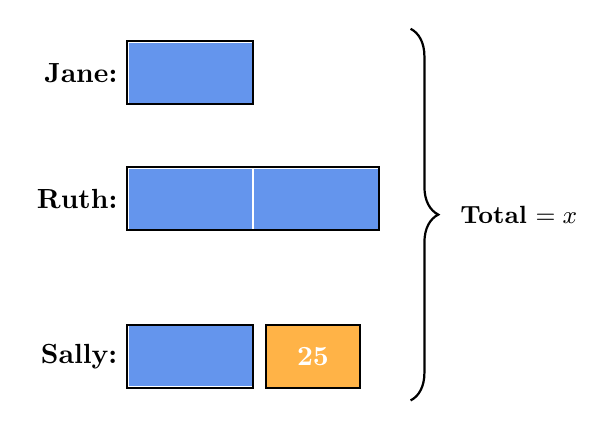
\begin{tikzpicture}[scale=0.8, every node/.style={font=\small}]
    % Jane: 1 kotak
    \node[anchor=east, font=\bfseries] at (0, 3) {Jane:};
    \draw[fill=colP, draw=white, line width=1pt] (0, 2.5) rectangle (2, 3.5);
    \draw[thick] (0, 2.5) rectangle (2, 3.5); % Border luar
    \node[white, font=\bfseries] at (1, 3) {};
    
    % Ruth: 2 kotak
    \node[anchor=east, font=\bfseries] at (0, 1) {Ruth:};
    \foreach \x in {0, 2} {
        \draw[fill=colP, draw=white, line width=1pt] (\x, 0.5) rectangle (\x+2, 1.5);
    }
    \draw[thick] (0, 0.5) rectangle (4, 1.5); % Border luar
    \node[white, font=\bfseries] at (1, 1) {};
    \node[white, font=\bfseries] at (3, 1) {};
    
    % Sally: 1 kotak + 25
    \node[anchor=east, font=\bfseries] at (0, -1.5) {Sally:};
    \draw[fill=colP, draw=white, line width=1pt] (0, -2) rectangle (2, -1);
    \draw[thick] (0, -2) rectangle (2, -1);
    \node[white, font=\bfseries] at (1, -1.5) {};
    
    % Bagian +25 (beda warna/ukuran)
    \draw[fill=colQ, draw=black, thick] (2.2, -2) rectangle (3.7, -1) node[midway, white, font=\bfseries] {25};
    
    % Total Brace
    \draw[decorate,decoration={brace,amplitude=10pt,mirror},thick] (4.5, -2.2) -- (4.5, 3.7) node[midway, right=0.5cm, align=left] {\textbf{Total} $= x$};
\end{tikzpicture}
\end{center}

Terlihat total unit kotak biru ada 4 buah.
\[ x = 4 \text{ kotak} + 25 \]

\textbf{(a) Menyatakan Jane dalam $x$}
Karena Jane memiliki tepat 1 kotak (1 unit):
\begin{align*}
    4 \text{ unit} + 25 &= x \\
    4 \text{ unit} &= x - 25 \\
    1 \text{ unit} &= \frac{x - 25}{4}
\end{align*}
Jadi, permen Jane = $\boxed{\frac{x - 25}{4}}$.

\textbf{(b) Jika $x = 265$}
\begin{align*}
    4 \text{ unit} &= 265 - 25 \\
    4 \text{ unit} &= 240 \\
    1 \text{ unit} &= 60
\end{align*}

Maka:
\begin{itemize}
    \item \textbf{Jane} (1 unit) = \textbf{60}
    \item \textbf{Ruth} (2 unit) = $60 \times 2$ = \textbf{120}
    \item \textbf{Sally} (1 unit + 25) = $60 + 25$ = \textbf{85}
\end{itemize}

\newpage

\subsection*{Soal 2: Perbandingan (Ratio)}

\textbf{Soal:}
Kota P memiliki $\frac{2}{5}$ jumlah penduduk Kota Q. Perbandingan jumlah penduduk di Kota R terhadap Kota P adalah $4:7$. Kota Q memiliki 8100 penduduk lebih banyak daripada Kota R. Berapa jumlah penduduk di Kota R?

\hrulefill

\textbf{Pembahasan:}

Kita perlu menyamakan "ukuran kotak" (unit) untuk Kota P agar bisa membandingkan ketiga kota.
\begin{itemize}
    \item P : Q = 2 : 5 (Kalikan 7) $\rightarrow$ P : Q = 14 : 35
    \item R : P = 4 : 7 (Kalikan 2) $\rightarrow$ R : P = 8 : 14
\end{itemize}
Sekarang unit P sudah sama (14 unit).

\begin{center}
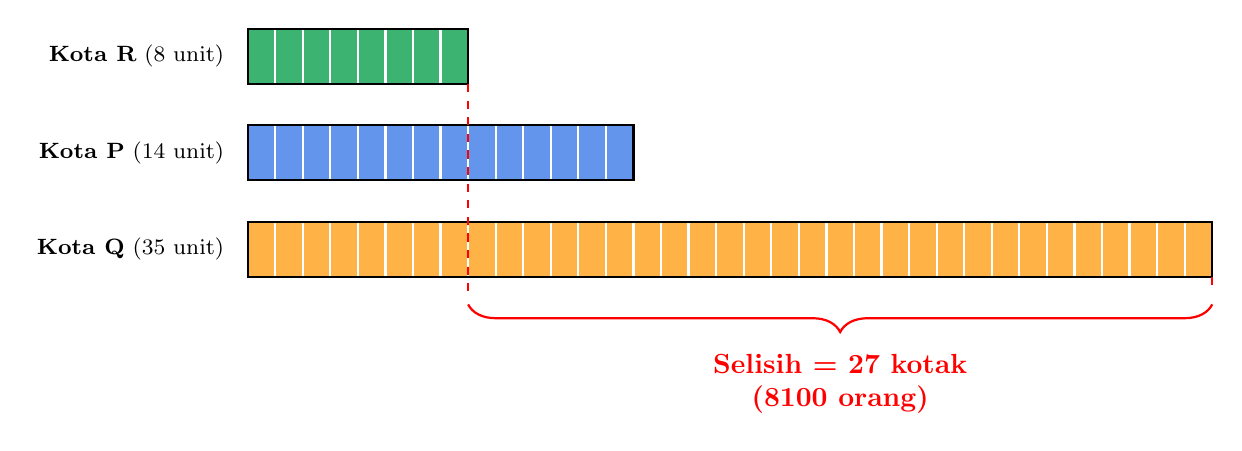
\begin{tikzpicture}[scale=0.35, every node/.style={font=\footnotesize}]
    % R (8 unit)
    \node[anchor=east] at (-0.5, 7) {\textbf{Kota R} (8 unit)};
    \draw[fill=colR] (0, 6) rectangle (8, 8);
    \foreach \x in {1,...,7} \draw[white, line width=0.8pt] (\x, 6) -- (\x, 8); % Grid lines
    \draw[thick] (0, 6) rectangle (8, 8); % Border
    
    % P (14 unit)
    \node[anchor=east] at (-0.5, 3.5) {\textbf{Kota P} (14 unit)};
    \draw[fill=colP] (0, 2.5) rectangle (14, 4.5);
    \foreach \x in {1,...,13} \draw[white, line width=0.8pt] (\x, 2.5) -- (\x, 4.5); % Grid lines
    \draw[thick] (0, 2.5) rectangle (14, 4.5); % Border
    
    % Q (35 unit)
    \node[anchor=east] at (-0.5, 0) {\textbf{Kota Q} (35 unit)};
    \draw[fill=colQ] (0, -1) rectangle (35, 1);
    \foreach \x in {1,...,34} \draw[white, line width=0.8pt] (\x, -1) -- (\x, 1); % Grid lines
    \draw[thick] (0, -1) rectangle (35, 1); % Border
    
    % Garis putus-putus penanda selisih
    \draw[dashed, red, thick] (8, 6) -- (8, -1.5);
    \draw[dashed, red, thick] (35, -1) -- (35, -1.5);
    
    % Brace Selisih
    \draw[decorate,decoration={brace,amplitude=10pt,mirror},thick, red] (8, -2) -- (35, -2) 
    node[midway, below=0.5cm, align=center, font=\bfseries, color=red] {Selisih = 27 kotak\\(8100 orang)};
\end{tikzpicture}
\end{center}

Dari gambar grid di atas:
Selisih panjang batang Q dan R adalah $35 - 8 = 27$ kotak.

\[ 27 \text{ unit} = 8100 \implies 1 \text{ unit} = 300 \]

\textbf{Kota R (8 unit):}
\[ 8 \times 300 = \mathbf{2.400} \text{ penduduk} \]

\newpage

\subsection*{Soal 3: Kecepatan (Speed)}

\textbf{Soal:}
Nathaniel dan Trevor masing-masing lari santai (joging) dari Taman E ke Taman F. Nathaniel membutuhkan waktu 2 jam untuk menempuh seluruh perjalanan, sedangkan Trevor membutuhkan waktu 1 jam untuk menempuh tiga perlima perjalanan tersebut. Tentukan rasio kecepatan rata-rata Nathaniel terhadap kecepatan rata-rata Trevor.

\hrulefill

\textbf{Pembahasan:}

Kita bandingkan \textbf{jarak yang ditempuh dalam waktu yang sama}, yaitu 1 jam.
Kita anggap Jarak Total = 10 unit jarak (KPK dari 2 dan 5 untuk mempermudah visualisasi).

\begin{center}
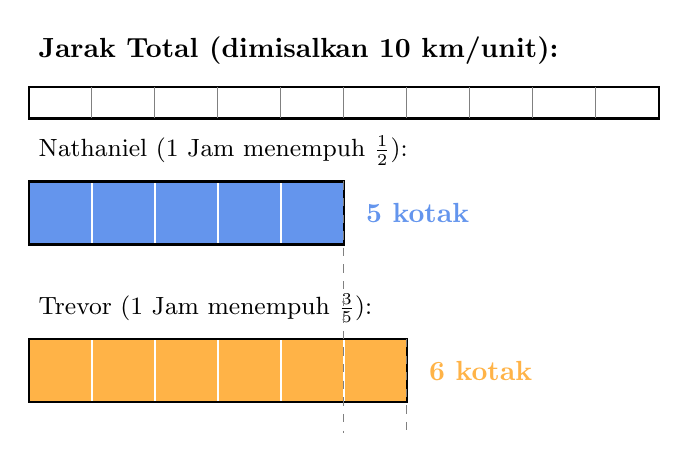
\begin{tikzpicture}[scale=0.8, every node/.style={font=\small}]
    % --- Header Jarak Total ---
    \node[anchor=south west, font=\bfseries] at (0, 6.2) {Jarak Total (dimisalkan 10 km/unit):};
    % Kotak Jarak Total (Kosong/Grid)
    \draw[thick] (0, 5.5) rectangle (10, 6);
    \foreach \x in {1,...,9} \draw[gray] (\x, 5.5) -- (\x, 6);
    
    % --- Nathaniel ---
    \node[anchor=south west] at (0, 4.6) {Nathaniel (1 Jam menempuh $\frac{1}{2}$):};
    % Batang Nathaniel (5 kotak)
    \draw[fill=colP] (0, 3.5) rectangle (5, 4.5);
    \foreach \x in {1,...,4} \draw[white, line width=0.8pt] (\x, 3.5) -- (\x, 4.5);
    \draw[thick] (0, 3.5) rectangle (5, 4.5); % Border
    % Label Jumlah Kotak
    \node[right, colP, font=\bfseries] at (5.2, 4) {5 kotak};

    % --- Trevor ---
    \node[anchor=south west] at (0, 2.1) {Trevor (1 Jam menempuh $\frac{3}{5}$):};
    % Batang Trevor (6 kotak)
    \draw[fill=colQ] (0, 1) rectangle (6, 2);
    \foreach \x in {1,...,5} \draw[white, line width=0.8pt] (\x, 1) -- (\x, 2);
    \draw[thick] (0, 1) rectangle (6, 2); % Border
    % Label Jumlah Kotak
    \node[right, colQ, font=\bfseries] at (6.2, 1.5) {6 kotak};
    
    % --- Garis Bantu ---
    \draw[dashed, gray] (5, 4.5) -- (5, 0.5); % Garis batas Nathaniel
    \draw[dashed, gray] (6, 2) -- (6, 0.5);    % Garis batas Trevor
\end{tikzpicture}
\end{center}

Rasio Kecepatan = Rasio Jarak (dalam 1 jam)
\[ \text{Nathaniel} : \text{Trevor} = 5 \text{ kotak} : 6 \text{ kotak} = \mathbf{5 : 6} \]

\newpage

\subsection*{Soal 4: Rasio Bertingkat (Ratio)}

\textbf{Soal:}
Rasio jumlah buku Claude terhadap buku Robin adalah $5:6$. Rasio jumlah buku Robin terhadap buku Ian adalah $7:4$. Jika Claude memiliki 22 buku lebih banyak daripada Ian, berapa banyak buku yang dimiliki Robin?

\hrulefill

\textbf{Pembahasan:}

Variabel penghubung adalah **Robin**. Kita harus menyamakan unit Robin pada kedua rasio.
\begin{itemize}
    \item C : R = 5 : 6 (Kalikan 7) $\rightarrow$ \textbf{35 : 42}
    \item R : I = 7 : 4 (Kalikan 6) $\rightarrow$ \textbf{42 : 24}
\end{itemize}
Rasio gabungan C : R : I = 35 : 42 : 24.

\begin{center}
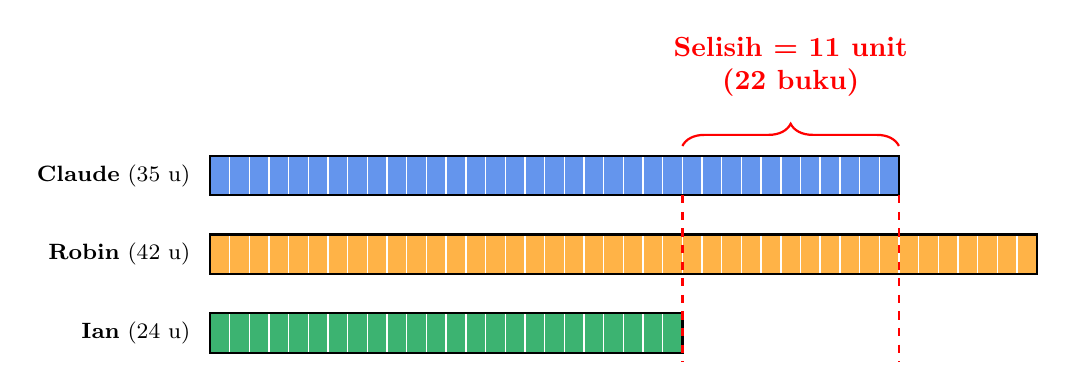
\begin{tikzpicture}[scale=0.25, every node/.style={font=\footnotesize}]
    % Claude (35 unit)
    \node[anchor=east] at (-0.5, 8) {\textbf{Claude} (35 u)};
    \draw[fill=colP] (0, 7) rectangle (35, 9);
    \foreach \x in {1,...,34} \draw[white, line width=0.5pt] (\x, 7) -- (\x, 9); % Grid halus
    \draw[thick] (0, 7) rectangle (35, 9);
    
    % Robin (42 unit)
    \node[anchor=east] at (-0.5, 4) {\textbf{Robin} (42 u)};
    \draw[fill=colQ] (0, 3) rectangle (42, 5);
    \foreach \x in {1,...,41} \draw[white, line width=0.5pt] (\x, 3) -- (\x, 5);
    \draw[thick] (0, 3) rectangle (42, 5);
    
    % Ian (24 unit)
    \node[anchor=east] at (-0.5, 0) {\textbf{Ian} (24 u)};
    \draw[fill=colR] (0, -1) rectangle (24, 1);
    \foreach \x in {1,...,23} \draw[white, line width=0.5pt] (\x, -1) -- (\x, 1);
    \draw[thick] (0, -1) rectangle (24, 1);
    
    % Penanda Selisih
    \draw[dashed, red, thick] (24, 7) -- (24, -1.5);
    \draw[dashed, red, thick] (35, 7) -- (35, -1.5);
    
    \draw[decorate,decoration={brace,amplitude=8pt},thick, red] (24, 9.5) -- (35, 9.5) 
    node[midway, above=0.5cm, align=center, font=\bfseries, color=red] {Selisih = 11 unit\\(22 buku)};
\end{tikzpicture}
\end{center}

Selisih unit Claude dan Ian: $35 - 24 = 11$ unit.
\[ 11 \text{ unit} = 22 \text{ buku} \implies 1 \text{ unit} = 2 \text{ buku} \]

\textbf{Jumlah buku Robin (42 unit):}
\[ 42 \times 2 = \mathbf{84} \text{ buku} \]

\newpage

\subsection*{Soal 5: Pecahan Sisa (Fraction of Remainder)}

\textbf{Soal:}
Gavin memiliki sejumlah uang. Ia menyumbangkan $\frac{1}{2}$ dari uangnya ke Yayasan A. Kemudian, ia menyumbangkan $\frac{1}{4}$ dari sisanya ke Palang Merah. Selanjutnya, ia memberikan $\frac{1}{3}$ dari sisanya lagi ke Mercy Corps. Terakhir, ia mendonasikan $\frac{1}{2}$ dari sisanya ke Global Fund. Gavin tersisa \$625 pada akhirnya. Berapa uang Gavin mula-mula?

\hrulefill

\textbf{Pembahasan (Working Backwards):}

Kita gambar kotaknya secara harfiah untuk melihat sisa dengan metode mundur.

\begin{center}
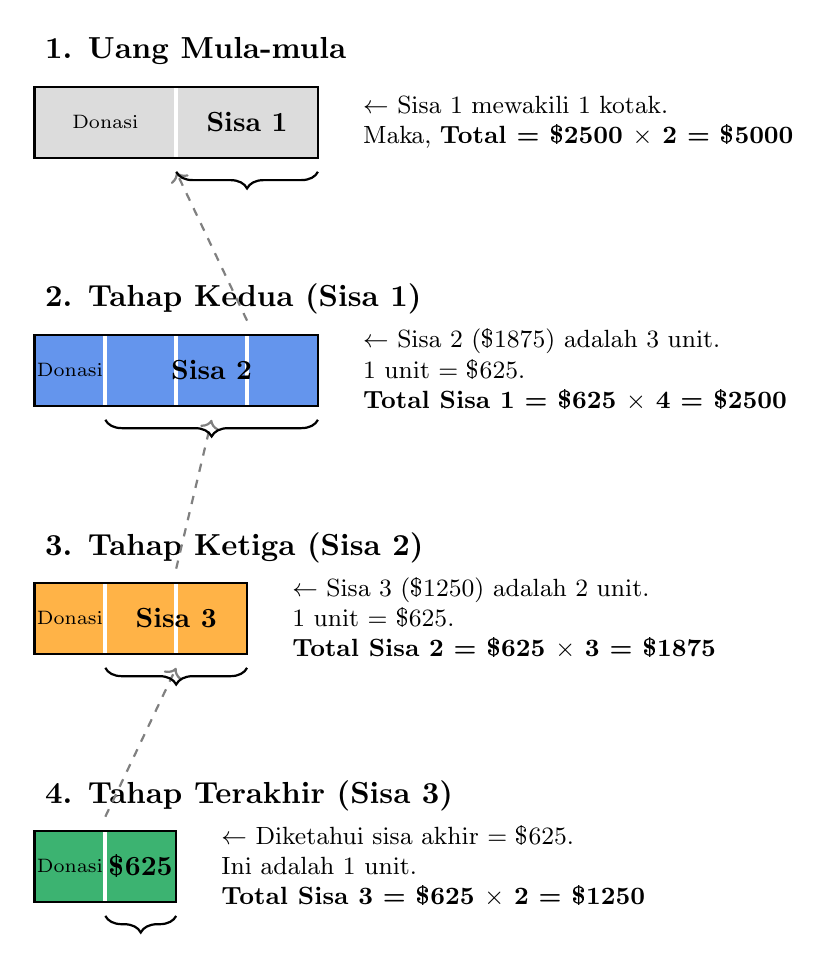
\begin{tikzpicture}[scale=0.9, every node/.style={font=\small}]
    % --- Bar 4: Sisa 3 ---
    \node[anchor=west, font=\bfseries, scale=1.1] at (0, 1.5) {4. Tahap Terakhir (Sisa 3)};
    % Sisa akhir 1/2 bagian. Kita gambar Sisa 3 sebagai 2 kotak.
    \draw[fill=colR] (0, 0) rectangle (2, 1);
    \draw[white, line width=1.5pt] (1, 0) -- (1, 1);
    \draw[thick] (0, 0) rectangle (2, 1);
    
    \node at (0.5, 0.5) {\scriptsize Donasi};
    \node[font=\bfseries] at (1.5, 0.5) {\$625};
    
    % Brace Sisa Akhir
    \draw[decorate,decoration={brace,amplitude=6pt,mirror},thick] (1, -0.2) -- (2, -0.2);
    
    % Penjelasan Kanan
    \node[right, align=left] at (2.5, 0.5) {
        $\leftarrow$ Diketahui sisa akhir = \$625.\\
        Ini adalah 1 unit.\\
        \textbf{Total Sisa 3 = \$625 $\times$ 2 = \$1250}
    };

    % Panah penghubung ke atas
    \draw[dashed, ->, thick, gray] (1, 1.2) -- (2, 3.3);

    % --- Bar 3: Sisa 2 ---
    \node[anchor=west, font=\bfseries, scale=1.1] at (0, 5) {3. Tahap Ketiga (Sisa 2)};
    % Sisa 3 mewakili 2/3 bagian (karena 1/3 didonasikan).
    % Kita gambar Sisa 2 sebagai 3 kotak.
    \draw[fill=colQ] (0, 3.5) rectangle (3, 4.5);
    \foreach \x in {1,2} \draw[white, line width=1.5pt] (\x, 3.5) -- (\x, 4.5);
    \draw[thick] (0, 3.5) rectangle (3, 4.5);
    
    \node at (0.5, 4) {\scriptsize Donasi};
    \node[font=\bfseries] at (2, 4) {Sisa 3};
    
    % Brace Sisa 3 (Mencakup 2 kotak kanan)
    \draw[decorate,decoration={brace,amplitude=6pt,mirror},thick] (1, 3.3) -- (3, 3.3);
    
    % Penjelasan Kanan
    \node[right, align=left] at (3.5, 4) {
        $\leftarrow$ Sisa 3 (\$1250) adalah 2 unit.\\
        1 unit = \$625.\\
        \textbf{Total Sisa 2 = \$625 $\times$ 3 = \$1875}
    };

    % Panah penghubung ke atas
    \draw[dashed, ->, thick, gray] (2, 4.7) -- (2.5, 6.8);

    % --- Bar 2: Sisa 1 ---
    \node[anchor=west, font=\bfseries, scale=1.1] at (0, 8.5) {2. Tahap Kedua (Sisa 1)};
    % Sisa 2 mewakili 3/4 bagian (karena 1/4 didonasikan).
    % Kita gambar Sisa 1 sebagai 4 kotak.
    \draw[fill=colP] (0, 7) rectangle (4, 8);
    \foreach \x in {1,2,3} \draw[white, line width=1.5pt] (\x, 7) -- (\x, 8);
    \draw[thick] (0, 7) rectangle (4, 8);
    
    \node at (0.5, 7.5) {\scriptsize Donasi};
    \node[font=\bfseries] at (2.5, 7.5) {Sisa 2};
    
    % Brace Sisa 2 (Mencakup 3 kotak kanan)
    \draw[decorate,decoration={brace,amplitude=6pt,mirror},thick] (1, 6.8) -- (4, 6.8);
    
    % Penjelasan Kanan
    \node[right, align=left] at (4.5, 7.5) {
        $\leftarrow$ Sisa 2 (\$1875) adalah 3 unit.\\
        1 unit = \$625.\\
        \textbf{Total Sisa 1 = \$625 $\times$ 4 = \$2500}
    };

    % Panah penghubung ke atas
    \draw[dashed, ->, thick, gray] (3, 8.2) -- (2, 10.3);

    % --- Bar 1: Mula-mula ---
    \node[anchor=west, font=\bfseries, scale=1.1] at (0, 12) {1. Uang Mula-mula};
    % Sisa 1 mewakili 1/2 bagian (karena 1/2 didonasikan). 
    % Artinya Mula-mula = 2 kotak.
    \draw[fill=colGrayMid, draw=black] (0, 10.5) rectangle (4, 11.5);
    \draw[white, line width=1.5pt] (2, 10.5) -- (2, 11.5);
    \draw[thick] (0, 10.5) rectangle (4, 11.5);
    
    \node at (1, 11) {\scriptsize Donasi};
    \node[font=\bfseries] at (3, 11) {Sisa 1};
    
    % Brace Sisa 1
    \draw[decorate,decoration={brace,amplitude=6pt,mirror},thick] (2, 10.3) -- (4, 10.3);
    
    % Penjelasan Kanan
    \node[right, align=left] at (4.5, 11) {
        $\leftarrow$ Sisa 1 mewakili 1 kotak.\\
        Maka, \textbf{Total = \$2500 $\times$ 2 = \$5000}
    };

\end{tikzpicture}
\end{center}

Jadi, uang Gavin mula-mula adalah \textbf{\$5.000}.

\newpage

% =================================================================================
% SOAL BAR MODEL 6-10
% =================================================================================
\section*{Latihan Soal Paket B (6-10)}

\subsection*{Soal 6: Bilangan Cacah (Quotient \& Remainder)}
\textbf{Soal:}
Ketika Bilangan X dibagi dengan Bilangan Y, hasil baginya adalah 16 dan sisanya 3. Jumlah dari kedua bilangan, hasil bagi, dan sisanya adalah 345. Berapakah Bilangan X?

\hrulefill

\textbf{Pembahasan:}

Dari soal, kita tahu hubungan: $X = (16 \times Y) + 3$.
Jika kita gambarkan dalam kotak unit:
\begin{itemize}
    \item \textbf{Bilangan Y} = 1 kotak unit.
    \item \textbf{Bilangan X} = 16 kotak unit + nilai 3.
\end{itemize}

Persamaan totalnya:
\[ X + Y + 16 + 3 = 345 \]
\[ (16 \text{ unit} + 3) + (1 \text{ unit}) + 19 = 345 \]
\[ 17 \text{ unit} + 22 = 345 \]
\[ 17 \text{ unit} = 323 \]

\vspace{0.5cm}
\begin{center}
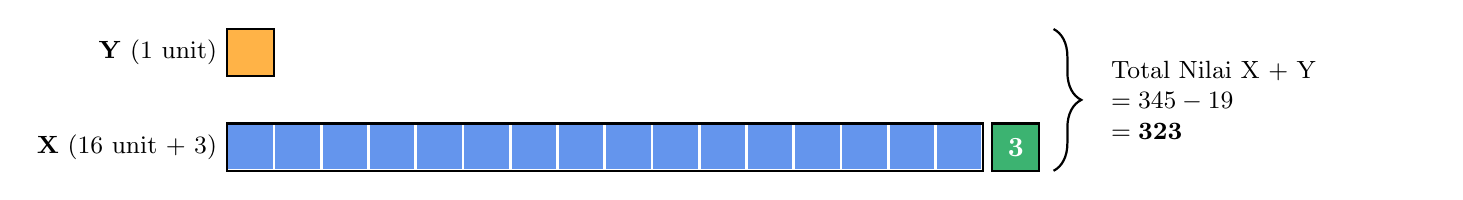
\begin{tikzpicture}[scale=0.6, every node/.style={font=\small}]
    % --- Bar Y ---
    \node[anchor=east] at (0, 3) {\textbf{Y} (1 unit)};
    \draw[fill=colOrange, draw=white, line width=1pt] (0, 2.5) rectangle (1, 3.5);
    \draw[thick] (0, 2.5) rectangle (1, 3.5); % Border
    \node at (0.5, 3) {};

    % --- Bar X ---
    \node[anchor=east] at (0, 1) {\textbf{X} (16 unit + 3)};
    % Loop menggambar 16 kotak biru
    \foreach \x in {0, ..., 15} {
        \draw[fill=colBlue, draw=white, line width=1pt] (\x, 0.5) rectangle (\x+1, 1.5);
    }
    \draw[thick] (0, 0.5) rectangle (16, 1.5); % Border luar unit
    
    % Kotak sisa 3 (Beda warna & ukuran fix visual)
    \draw[fill=colGreen, draw=black, thick] (16.2, 0.5) rectangle (17.2, 1.5);
    \node[white, font=\bfseries] at (16.7, 1) {3};

    % Label Unit
    \node[white] at (0.5, 1) {};
    \node[white] at (15.5, 1) {};
    \node at (8, 1) {};

    % Brace Total
    \draw[decorate,decoration={brace,amplitude=10pt,mirror},thick] (17.5, 0.5) -- (17.5, 3.5) 
    node[midway, right=0.6cm, align=left, text width=4cm] {Total Nilai X + Y\\$= 345 - 19$\\$= \mathbf{323}$};
\end{tikzpicture}
\end{center}
\vspace{0.5cm}

\textbf{Hitungan:}
\[ 1 \text{ unit} = 323 \div 17 = 19 \quad (\text{Nilai Y}) \]
\[ X = (16 \times 19) + 3 = 304 + 3 = \mathbf{307} \]

\newpage

\subsection*{Soal 7: Pecahan (Equal Fractions)}
\textbf{Soal:}
Di Peternakan A, $\frac{4}{5}$ dari jumlah domba sama dengan $\frac{1}{2}$ dari jumlah domba di Peternakan B. Total domba di Peternakan A dan Peternakan B adalah 845 ekor. Berapa jumlah domba di Peternakan B?

\hrulefill

\textbf{Pembahasan:}

Samakan pembilang pecahan agar unit pembandingnya setara (Equal Units).
\begin{itemize}
    \item Peternakan A: $\frac{4}{5}$ (4 kotak dari total 5).
    \item Peternakan B: $\frac{1}{2} = \frac{4}{8}$ (4 kotak dari total 8).
\end{itemize}
Jadi, kita gambar 4 kotak yang "sama besar" untuk kedua peternakan sebagai jembatan.

\vspace{0.5cm}
\begin{center}
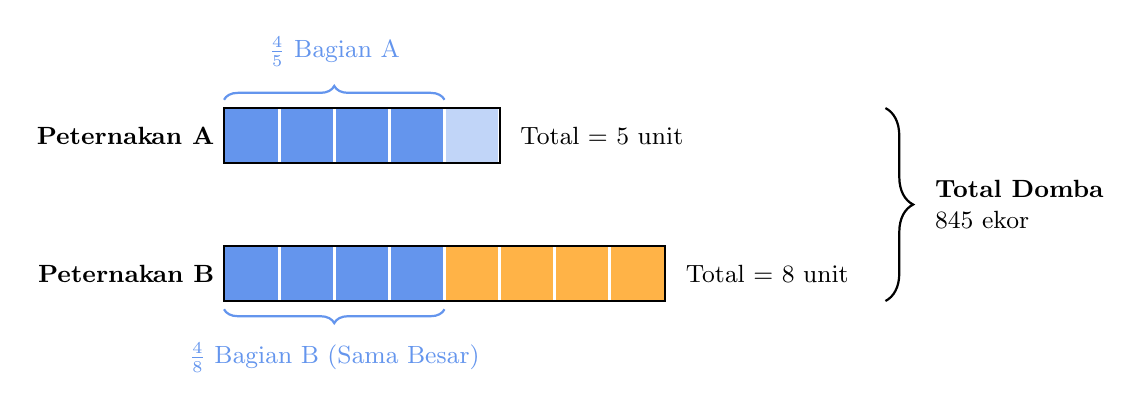
\begin{tikzpicture}[scale=0.7, every node/.style={font=\small}]
    % --- Peternakan A ---
    \node[anchor=east] at (0, 4) {\textbf{Peternakan A}};
    % 4 Unit Setara (Biru)
    \foreach \x in {0, ..., 3} {
        \draw[fill=colBlue, draw=white, line width=1pt] (\x, 3.5) rectangle (\x+1, 4.5);
    }
    % 1 Unit Sisa (Biru Muda - bagian dari total A)
    \draw[fill=colBlue!40, draw=white, line width=1pt] (4, 3.5) rectangle (5, 4.5);
    \draw[thick] (0, 3.5) rectangle (5, 4.5); % Border
    \node[right] at (5.2, 4) {Total = 5 unit};

    % --- Peternakan B ---
    \node[anchor=east] at (0, 1.5) {\textbf{Peternakan B}};
    % 4 Unit Setara (Biru) - Sejajar dengan atas
    \foreach \x in {0, ..., 3} {
        \draw[fill=colBlue, draw=white, line width=1pt] (\x, 1) rectangle (\x+1, 2);
    }
    % 4 Unit Sisa (Oranye - total B ada 8)
    \foreach \x in {4, ..., 7} {
        \draw[fill=colOrange, draw=white, line width=1pt] (\x, 1) rectangle (\x+1, 2);
    }
    \draw[thick] (0, 1) rectangle (8, 2); % Border
    \node[right] at (8.2, 1.5) {Total = 8 unit};

    % Brace Hubungan (Atas & Bawah)
    \draw[decorate,decoration={brace,amplitude=5pt,raise=3pt}, thick, color=colBlue] (0, 4.5) -- (4, 4.5) node[midway, above=0.4cm] {$\frac{4}{5}$ Bagian A};
    \draw[decorate,decoration={brace,amplitude=5pt,mirror,raise=3pt}, thick, color=colBlue] (0, 1) -- (4, 1) node[midway, below=0.4cm] {$\frac{4}{8}$ Bagian B (Sama Besar)};

    % Brace Total Keseluruhan (DI KANAN)
    % Menjangkau dari bawah B (y=1) sampai atas A (y=4.5)
    \draw[decorate,decoration={brace,amplitude=10pt,mirror}, thick] (12, 1) -- (12, 4.5) 
    node[midway, right=0.5cm, align=left] {\textbf{Total Domba}\\845 ekor};

\end{tikzpicture}
\end{center}
\vspace{0.5cm}

\textbf{Hitungan:}
Total seluruh kotak unit = 5 (A) + 8 (B) = 13 unit.
\[ 13 \text{ unit} = 845 \]
\[ 1 \text{ unit} = 845 \div 13 = 65 \text{ ekor} \]
Peternakan B memiliki 8 unit:
\[ 8 \times 65 = \mathbf{520} \text{ ekor} \]

\newpage

\subsection*{Soal 8: Rasio (Before and After)}
\textbf{Soal:}
Rasio uang Terry terhadap uang Maria awalnya adalah 4:9. Setelah Terry membelanjakan setengah uangnya dan Maria membelanjakan \$20, uang Maria menjadi dua kali lipat uang Terry. Berapa uang Terry mula-mula?

\hrulefill

\textbf{Pembahasan:}

Gunakan kotak unit untuk melacak perubahan.
\begin{itemize}
    \item \textbf{Awal:} Terry (4 kotak), Maria (9 kotak).
    \item \textbf{Aksi:} Terry sisa 2 kotak (karena setengahnya habis).
    \item \textbf{Syarat Akhir:} Uang Maria = 2 $\times$ Uang Terry. 
    Karena sisa Terry adalah 2 kotak, maka sisa Maria haruslah $2 \times 2 = \mathbf{4 \text{ kotak}}$.
\end{itemize}

\vspace{0.5cm}
\begin{center}
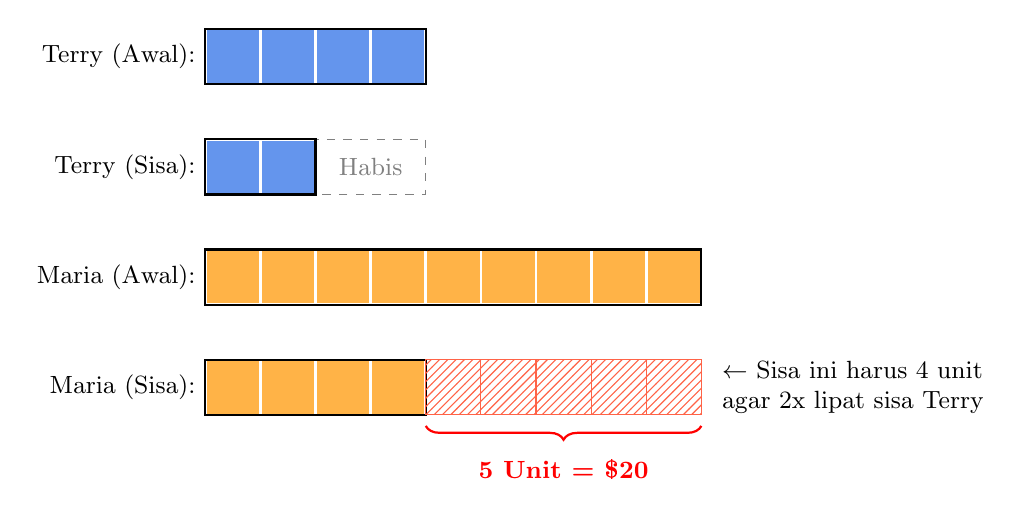
\begin{tikzpicture}[scale=0.7, every node/.style={font=\small}]
    % --- Terry Awal ---
    \node[anchor=east] at (0, 6) {Terry (Awal):};
    \foreach \x in {0, ..., 3} {
        \draw[fill=colBlue, draw=white, line width=1pt] (\x, 5.5) rectangle (\x+1, 6.5);
    }
    \draw[thick] (0, 5.5) rectangle (4, 6.5); 

    % --- Terry Akhir ---
    \node[anchor=east] at (0, 4) {Terry (Sisa):};
    % 2 Kotak Sisa
    \foreach \x in {0, 1} {
        \draw[fill=colBlue, draw=white, line width=1pt] (\x, 3.5) rectangle (\x+1, 4.5);
    }
    % 2 Kotak Hilang (Dashed)
    \draw[dashed, draw=gray] (2, 3.5) rectangle (4, 4.5);
    \node[gray] at (3, 4) {Habis};
    \draw[thick] (0, 3.5) rectangle (2, 4.5); % Border sisa

    % --- Maria Awal ---
    \node[anchor=east] at (0, 2) {Maria (Awal):};
    \foreach \x in {0, ..., 8} {
        \draw[fill=colOrange, draw=white, line width=1pt] (\x, 1.5) rectangle (\x+1, 2.5);
    }
    \draw[thick] (0, 1.5) rectangle (9, 2.5);

    % --- Maria Akhir ---
    \node[anchor=east] at (0, 0) {Maria (Sisa):};
    % 4 Kotak Sisa (Target)
    \foreach \x in {0, ..., 3} {
        \draw[fill=colOrange, draw=white, line width=1pt] (\x, -0.5) rectangle (\x+1, 0.5);
    }
    \draw[thick] (0, -0.5) rectangle (4, 0.5);
    
    % 5 Kotak Hilang ($20)
    \foreach \x in {4, ..., 8} {
        \draw[pattern=north east lines, pattern color=colRed, draw=colRed] (\x, -0.5) rectangle (\x+1, 0.5);
    }
    
    % Brace Penjelasan Logika
    \draw[decorate,decoration={brace,amplitude=5pt,mirror}, thick, red] (4, -0.7) -- (9, -0.7) 
    node[midway, below=0.3cm] {\textbf{5 Unit = \$20}};
    
    \node[right, align=left] at (9.2, 0) {$\leftarrow$ Sisa ini harus 4 unit\\agar 2x lipat sisa Terry};

\end{tikzpicture}
\end{center}
\vspace{0.5cm}

\textbf{Hitungan:}
Dari gambar Maria (Akhir), selisih kotak awal (9) dan kotak sisa (4) adalah 5 kotak.
5 kotak ini mewakili uang yang dibelanjakan (\$20).
\[ 5 \text{ kotak} = \$20 \implies 1 \text{ kotak} = \$4 \]
Uang Terry Mula-mula (4 kotak):
\[ 4 \times \$4 = \mathbf{\$16} \]

\newpage

\subsection*{Soal 9: Perbandingan Dua Skenario (Gap \& Difference)}
\textbf{Soal:}
Ryan dan Marie memiliki sejumlah kelereng. 
\begin{itemize}
    \item \textbf{Skenario 1:} Jika Ryan kehilangan 15 kelereng, rasionya Ryan:Marie = 4:1.
    \item \textbf{Skenario 2:} Jika Ryan kehilangan 75 kelereng, rasionya Ryan:Marie = 3:2.
\end{itemize}
Berapa banyak kelereng Ryan mula-mula?

\hrulefill

\textbf{Pembahasan:}

Jumlah kelereng Marie **TETAP**. Kita jadikan Marie sebagai patokan unit yang sama.
\begin{itemize}
    \item Skenario 1: Ryan : Marie = 4 : 1. (Ubah jadi \textbf{8 : 2} agar Marie sama dengan skenario 2).
    \item Skenario 2: Ryan : Marie = \textbf{3 : 2}.
\end{itemize}
Jadi, kita gunakan **2 kotak** untuk Marie di kedua gambar.

\vspace{0.5cm}
\begin{center}
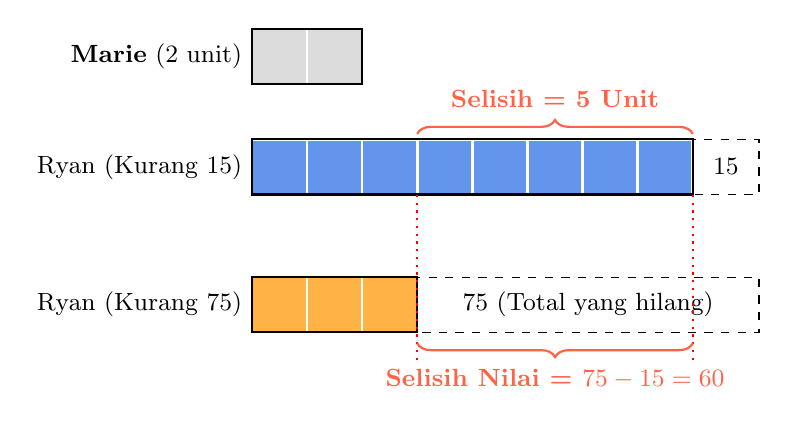
\begin{tikzpicture}[scale=0.7, every node/.style={font=\small}]
    % --- Marie (Konstan) ---
    \node[anchor=east] at (0, 6) {\textbf{Marie} (2 unit)};
    \foreach \x in {0, 1} {
        \draw[fill=colGray, draw=white, line width=1pt] (\x, 5.5) rectangle (\x+1, 6.5);
    }
    \draw[thick] (0, 5.5) rectangle (2, 6.5);

    % --- Ryan Skenario 1 ---
    \node[anchor=east] at (0, 4) {Ryan (Kurang 15)};
    % 8 Unit
    \foreach \x in {0, ..., 7} {
        \draw[fill=colBlue, draw=white, line width=1pt] (\x, 3.5) rectangle (\x+1, 4.5);
    }
    \draw[thick] (0, 3.5) rectangle (8, 4.5);
    % Kotak putus-putus +15 (Posisi relatif di kanan)
    \draw[dashed] (8, 3.5) rectangle (9.2, 4.5);
    \node at (8.6, 4) {15};

    % --- Ryan Skenario 2 ---
    \node[anchor=east] at (0, 1.5) {Ryan (Kurang 75)};
    % 3 Unit
    \foreach \x in {0, ..., 2} {
        \draw[fill=colOrange, draw=white, line width=1pt] (\x, 1) rectangle (\x+1, 2);
    }
    \draw[thick] (0, 1) rectangle (3, 2);
    % Kotak putus-putus +75
    \draw[dashed] (3, 1) rectangle (9.2, 2);
    \node at (6.1, 1.5) {75 (Total yang hilang)};

    % --- Analisis GAP ---
    % Garis bantu vertikal
    \draw[dotted, thick, red] (3, 0.5) -- (3, 3.5);
    \draw[dotted, thick, red] (8, 0.5) -- (8, 3.5);
    
    % Brace Selisih Unit
    \draw[decorate,decoration={brace,amplitude=5pt}, thick, colRed] (3, 4.6) -- (8, 4.6) 
    node[midway, above=0.2cm] {\textbf{Selisih = 5 Unit}};
    
    % Brace Selisih Nilai
    \draw[decorate,decoration={brace,amplitude=5pt,mirror}, thick, colRed] (3, 0.8) -- (8, 0.8) 
    node[midway, below=0.2cm] {\textbf{Selisih Nilai = $75 - 15 = 60$}};

\end{tikzpicture}
\end{center}
\vspace{0.5cm}

\textbf{Hitungan:}
Dari gambar, terlihat perbedaan panjang kotak Ryan (5 unit) setara dengan perbedaan nilai kehilangan (60).
\[ 5 \text{ unit} = 60 \implies 1 \text{ unit} = 12 \]
Ryan Mula-mula (Lihat Skenario 1):
\[ (8 \text{ unit} \times 12) + 15 = 96 + 15 = \mathbf{111} \]

\newpage

\subsection*{Soal 10: Desimal \& Logika (Assumption Method)}
\textbf{Soal:}
Sebuah perusahaan transportasi mengirimkan 78 piring. Mereka dibayar \$1.50 untuk setiap piring yang terkirim utuh, namun harus membayar ganti rugi \$9.50 untuk setiap piring yang pecah. Jika perusahaan tersebut menerima total \$73, berapa banyak piring yang pecah?

\hrulefill

\textbf{Pembahasan:}

Kita gunakan \textit{Assumption Method} (Metode Pengandaian). Kita bandingkan kondisi "Sempurna" dengan kondisi "Nyata" menggunakan diagram batang.

\vspace{0.5cm}
\begin{center}
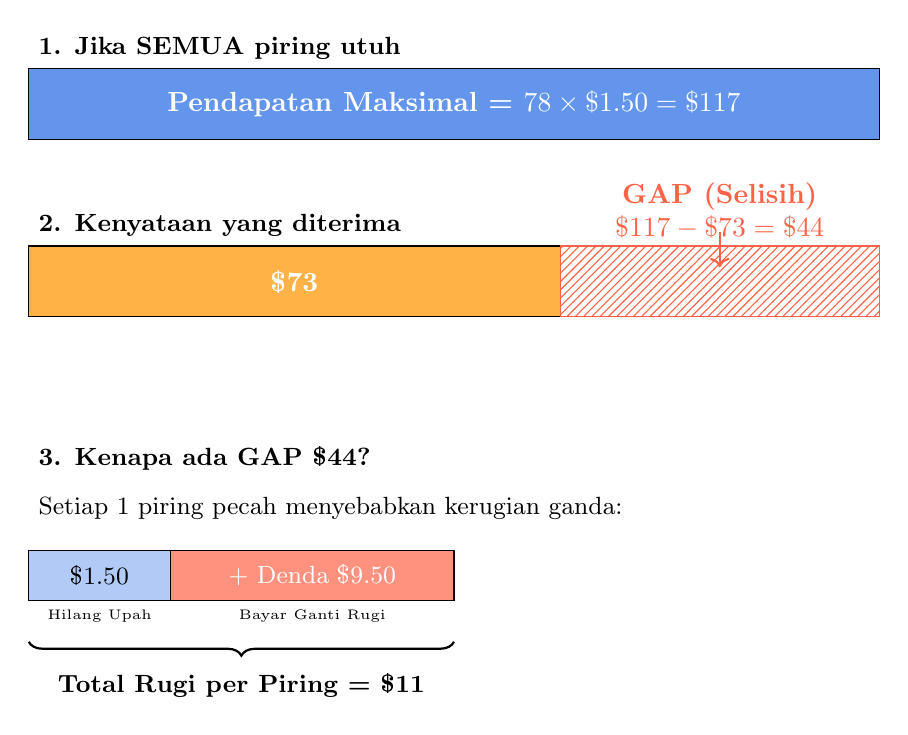
\begin{tikzpicture}[scale=0.9, every node/.style={font=\small}]
    % --- Bar 1: Harapan ---
    \node[anchor=south west] at (0, 3) {\textbf{1. Jika SEMUA piring utuh}};
    % Bar panjang (Biru)
    \draw[fill=colBlue, draw=black] (0, 2) rectangle (12, 3);
    \node[white, font=\bfseries] at (6, 2.5) {Pendapatan Maksimal = $78 \times \$1.50 = \$117$};

    % --- Bar 2: Kenyataan ---
    \node[anchor=south west] at (0, 0.5) {\textbf{2. Kenyataan yang diterima}};
    % Bar pendek (Oranye)
    \draw[fill=colOrange, draw=black] (0, -0.5) rectangle (7.5, 0.5);
    \node[white, font=\bfseries] at (3.75, 0) {\$73};

    % --- Bar Gap (Selisih) ---
    % Bar Arsiran Merah
    \draw[pattern=north east lines, pattern color=colRed, draw=colRed] (7.5, -0.5) rectangle (12, 0.5);
    \node[colRed, font=\bfseries, align=center] at (9.75, 1) {GAP (Selisih)\\$\$117 - \$73 = \$44$};
    \draw[->, thick, colRed] (9.75, 0.7) -- (9.75, 0.2); % Panah nunjuk ke gap

    % --- Penjelasan Unit Kerugian ---
    \node[anchor=west] at (0, -2.5) {\textbf{3. Kenapa ada GAP \$44?}};
    \node[anchor=west, align=left] at (0, -3.2) {Setiap 1 piring pecah menyebabkan kerugian ganda:};
    
    % Visualisasi 1 Unit Kerugian
    \draw[fill=colBlue!50, draw=black] (0, -4.5) rectangle (2, -3.8);
    \node at (1, -4.15) {\$1.50};
    \node[below, font=\tiny] at (1, -4.5) {Hilang Upah};
    
    \draw[fill=colRed!70, draw=black] (2, -4.5) rectangle (6, -3.8);
    \node[white] at (4, -4.15) {+ Denda \$9.50};
    \node[below, font=\tiny] at (4, -4.5) {Bayar Ganti Rugi};
    
    % Brace Total Rugi per Piring
    \draw[decorate,decoration={brace,amplitude=5pt,mirror,raise=15pt}, thick] (0, -4.5) -- (6, -4.5) 
    node[midway, below=0.8cm] {\textbf{Total Rugi per Piring = \$11}};

\end{tikzpicture}
\end{center}
\vspace{0.5cm}

\textbf{Hitungan:}
Total selisih uang (\$44) disebabkan oleh piring-piring yang pecah. Setiap satu piring pecah mengurangi total sebesar \$11.
\[ \text{Jumlah piring pecah} = \frac{\text{Total Selisih}}{\text{Rugi per Piring}} = \frac{44}{11} = \mathbf{4} \]

\end{document}
